% Created 2013-12-13 vie 12:20
\documentclass[11pt]{article}
%% \usepackage{fixltx2e}
\usepackage{graphicx}
\usepackage{xcolor}
%% \usepackage{longtable}
%% \usepackage{float}
%% \usepackage{wrapfig}
%% \usepackage{soul}
%% \usepackage{textcomp}
%% \usepackage{marvosym}
%% \usepackage{wasysym}
%% \usepackage{latexsym}
%% \usepackage{amssymb}
\usepackage{listings}
\usepackage[hidelinks,colorlinks=true,urlcolor=gray]{hyperref}
%% \tolerance=1000
%% \providecommand{\alert}[1]{[\textbf{#1}}

\usepackage[T1]{fontenc}
\usepackage[english]{babel}
\usepackage[utf8]{inputenc}
\usepackage{pifont}

% a command to highlight fields
\definecolor{shadecolor}{RGB}{205,205,205}
%\newcommand{\field}[1]{\noindent\colorbox{shadecolor}
%{\parbox{\dimexpr\textwidth-2\fboxsep\relax}{\textsc{#1}}}}
\newcommand{\field}[1]{\colorbox{shadecolor}{\small{\tt #1}}}
\newcommand{\code}[1]{\tt {\begingroup\escapechar-1 \expandafter\string\csname#1\endcsname\endgroup}}

%%%
%%%
%%%
\usepackage{parskip}
\setlength{\parindent}{15pt}
\setlength{\parskip}{2ex plus4mm minus3mm}
\usepackage{enumitem}
\setlist{nosep}
%\setlist[enumerate]{itemsep=0ex,topsep=0ex}
%\setlist[itemize]{itemsep=0ex,topsep=0ex}
%\setlist{noitemsep}
%%%
%%%
%%%

\title{\huge{\bf GUI Unit Testing (TUG) Framework}\\Testing Library and Project
  Wizard\\for Qt Panels} 

\author{\Large{ \bf Pedro Mateo}\\ {\large
    \tt pedromateo@um.es}\\ C\'atedra SAES} 

\date{\today} \hypersetup{
  pdfkeywords={}, pdfsubject={}, pdfcreator={Emacs Org-mode version
    7.9.3f}}

\begin{document}

%%%
%%% configuration for source code
\definecolor{lightgrey}{rgb}{0.91,0.91,0.91}
\newfont{\ttcustom}{cmtt9.5}

\lstset{ %
language=Java,                % choose the language of the code
basicstyle=\scriptsize \tt,       % the size of the fonts that are used for the code
numbers=left,                   % where to put the line-numbers
numberstyle=\tt \scriptsize,      % the size of the fonts that are used for the line-numbers
stepnumber=1,                   % the step between two line-numbers. If it's 1 each line will be numbered
numbersep=8pt,                  % how far the line-numbers are from the code
backgroundcolor=\color{lightgrey},  % choose the background color. You must add \usepackage{color}
showspaces=false,               % show spaces adding particular underscores
showstringspaces=false,         % underline spaces within strings
showtabs=false,                 % show tabs within strings adding particular underscores
frame=2px,                   % adds a frame around the code
tabsize=3,                      % sets default tabsize to 2 spaces
abovecaptionskip=-0.2\normalbaselineskip,
belowcaptionskip=\smallskipamount,
aboveskip=-0.2\normalbaselineskip,   
belowskip=\medskipamount, 
captionpos=t,                   % sets the caption-position to bottom
breaklines=true,                % sets automatic line breaking
breakatwhitespace=false,        % sets if automatic breaks should only happen at whitespace
title=\lstname,                 % show the filename of files included with \lstinputlisting; also try caption instead of title
escapeinside={\%*}{*)},          % if you want to add a comment within your code
keywordstyle=\color{black}          % keyword style
%morekeywords={*,...}            % if you want to add more keywords to the set
}

%%% end of configuration for source code
%%%



\maketitle
\setcounter{tocdepth}{3}
\tableofcontents
\vspace*{1cm}


\newpage



\section{Motivation}

\begin{flushright}
{\it TUG --- ``GUI Unit Testing'' --- ``Testing Unitario GUI'', in Spanish.}
\end{flushright}

TUG project~\footnote{The TUG Project is an initiative of C\'atedra
  SAES (\url{http://www.catedrasaes.org}) funded by the SAES company
  (\url{http://www.electronica-submarina.com}). This project and all
  its components have been designed and developed at University of
  Murcia (Spain).}
%
was born with the main purpose of providing a unit testing framework
for graphical user interfaces. The main goal was providing developers
with a method to easily create a battery of tests for Qt-based
applications. The tests had to simulate, as far as possible, users
interaction with the interface.

With this purpose, the TUG project is divided into two main components:
\begin{itemize}
%
\item {\bf TUG Wizard}: a wizard-like application that helps developers to
  create and configure, step by step, a test project aimed at testing a Qt
  based panel as well as the underlying model and communication classes (if
  they exists). It generates a new panel inheriting the original one. This
  new panel includes customized methods to simulate users interaction with
  the widgets composing the panel. It can also generate a full, standalone
  test project including testsuites and empty test methods ready for being
  filled with testing code.
%
\item {\bf TUG Base Library}: a library aimed at supporting the tests
  generated by TUG Wizard, as well as test projects created manually by
  developers. It provides a way to structure test suites, as well as a set
  of methods to support the definition of GUI tests, all around the Qt
  Test framework.
%
\end{itemize}

Along this document it is described how to properly use these
components to test your Qt-based projects.

%%% Local variables:
%%% mode: latex
%%% TeX-master: "README.tex"
%%% ispell-local-dictionary: "american"
%%% coding: utf-8
%%% fill-column: 75
%%% TeX-parse-self: t
%%% TeX-auto-save: t
%%% End:


\section{Package Content}

When uncompressing the TUG package you can find the following folders and
files:
%
\begin{itemize}
%
\item {\tt doc}: this folder includes this guide.
%
\item {\tt libTUG\_project}: this folder includes the C++ project of libTUG
  (GUI Unit Testing) library. Go to Section~\ref{sec:tuglib} for further
  information.
%
\item {\tt TUG\_wizard}: this folder includes the wizard application to
  create test projects (requires Java RE). Go to
  Section~\ref{sec:tugwizard} for further information.
%
\item {\tt install.sh}: this file can be used to install libTUG into a
  specific directory. Installation includes also the documentation and a
  tools folder including TUG Wizard. Type ``{\tt ./install.sh --help}'' to show
  further information. Maybe you need to provide execution permissions as
  follows: ``{\tt sudo chmod a+x install.sh}''.
%
\item {\tt README}: includes brief information about the package content.
%
\end{itemize}

%\label{sec:tugwizarddesignconfig}

%%% Local variables:
%%% mode: latex
%%% TeX-master: "README.tex"
%%% ispell-local-dictionary: "american"
%%% coding: utf-8
%%% fill-column: 75
%%% TeX-parse-self: t
%%% TeX-auto-save: t
%%% End:


\section{TUG Wizard Usage Guide}
\label{sec:tugwizard}


\subsection{Running TUG Wizard}

This section describes how to deploy TUG Wizard. Please, follow the steps
described in the following.

%\setcounter{enumi}{4}
\begin{enumerate}
%
%%% 
%%
\item {\bf Step 1: Unpack TUG package.}\\
%
  {\tt TUG Wizard} as well as
  {\tt TUGLib} are packed into a file named {\tt
    TUG\_vXX.tar.gz}. \\Unpack this package into a folder. As a result
  you will get a set of files as depicted in the figure below.

\vspace{1ex}
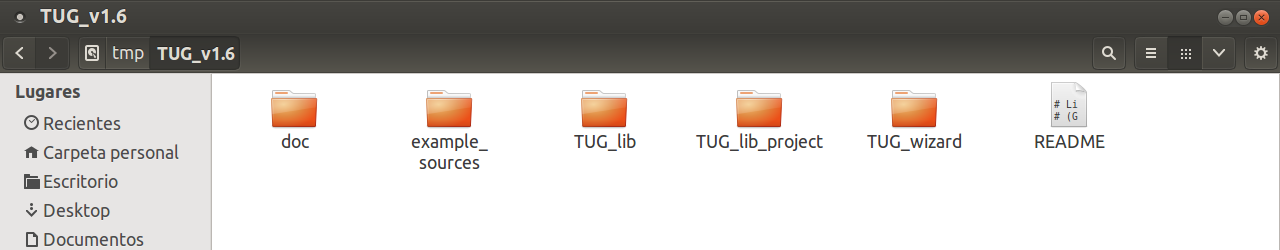
\includegraphics[width=.95\textwidth]{images/tug011.png}
\vspace{3ex}
%
%%% 
%%
\item {\bf Step 2: Launch TUG Wizard.}\\
%
  Go to {\tt TUG\_Wizard}
  folder. \\Add execution permission to the script file {\tt
    launch\_TUGWizard} as depicted in the figure below. \\Execute 
  {\tt launch\_TUGWizard} to launch the wizard prompt. 

\vspace{1ex}
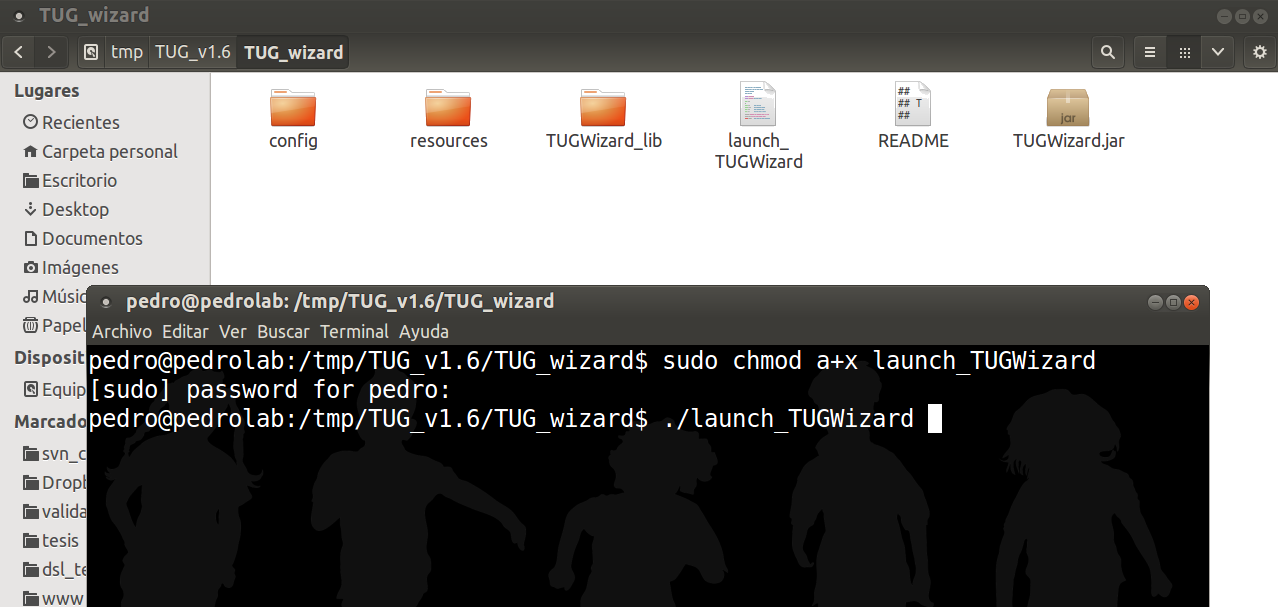
\includegraphics[width=.95\textwidth]{images/tug012.png}
\vspace{3ex}
\newpage
%
%%% 
%%
\item {\bf Step 3: TUG Wizard ready.}\\
%
  After the execution of the two
  steps described above, TUG Wizard will be prompted to start the
  configuration and generation of a testing project, as described in
  next section.

\vspace{1ex}
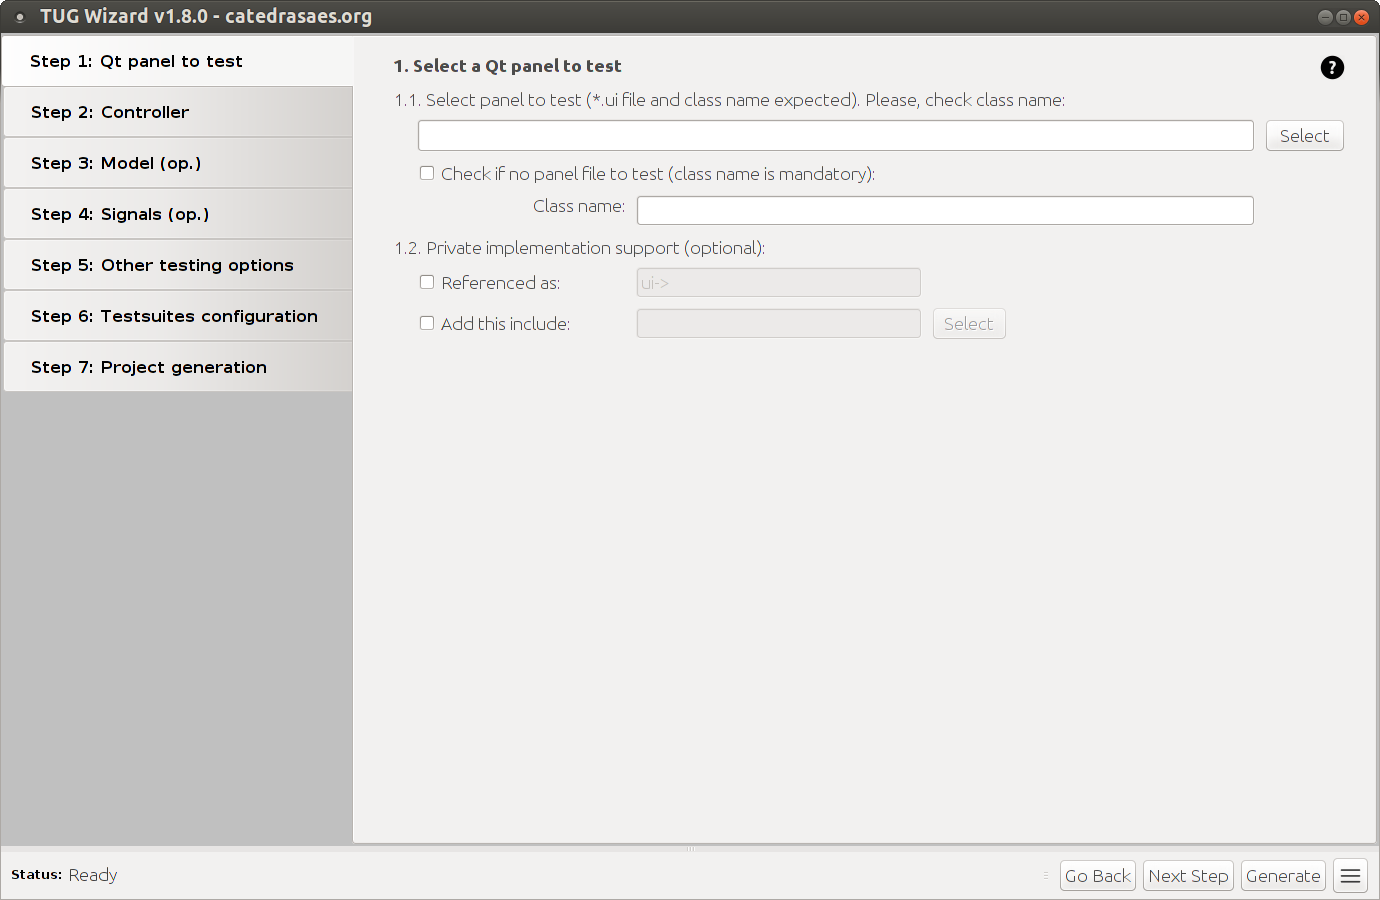
\includegraphics[width=.95\textwidth]{images/tug013.png}
\vspace{3ex}
\end{enumerate}
\newpage




%%% Local variables:
%%% mode: latex
%%% TeX-master: "README.tex"
%%% ispell-local-dictionary: "american"
%%% coding: utf-8
%%% fill-column: 75
%%% TeX-parse-self: t
%%% TeX-auto-save: t
%%% End:


\subsection{Test Projects in TUG Wizard}

TUG Wizard uses test projects that can be loaded from and saved to
files with extension {\tt *.tug}. Please, follow the steps described
in the following to load/save a TUG test project.

%\setcounter{enumi}{4}
\begin{enumerate}
%
%%% 
%%
\item {\bf Load a TUG project.}\\
%
  Click 
\includegraphics[width=.05\textwidth]{images/menu_icon.png} to
  deploy the pop-up menu and select \field{Load TUG project}.\\
%
  Select a {\tt *.tug} file and click \field{OK}. Data will be
  restored into TUG Wizard fields.


\vspace{1ex}
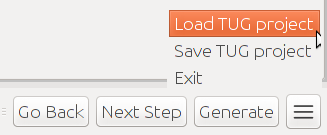
\includegraphics[width=.5\textwidth]{images/tug_load.png}

\vspace{1ex}
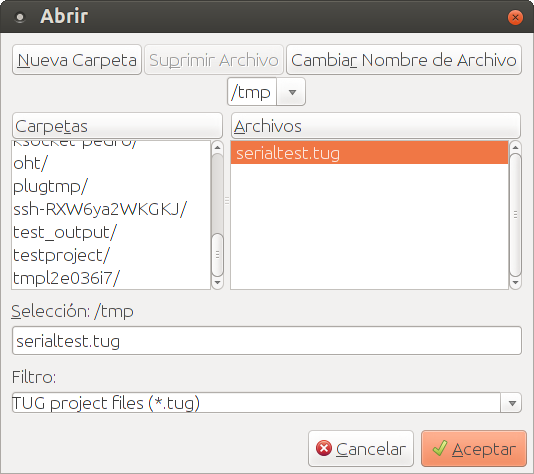
\includegraphics[width=.7\textwidth]{images/tug_load2.png}
\vspace{3ex}
\newpage

%
%%% 
%%
\item {\bf Save a TUG project.}\\
%
  Click 
\includegraphics[width=.05\textwidth]{images/menu_icon.png}
  to deploy the pop-up menu and select \field{Save TUG project}.\\
%
  Select a {\tt *.tug} file or write a new name for the project. Click
  \field{OK}. Data will be restored into TUG Wizard fields.


\vspace{1ex}
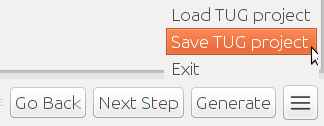
\includegraphics[width=.5\textwidth]{images/tug_save.png}

\vspace{1ex}
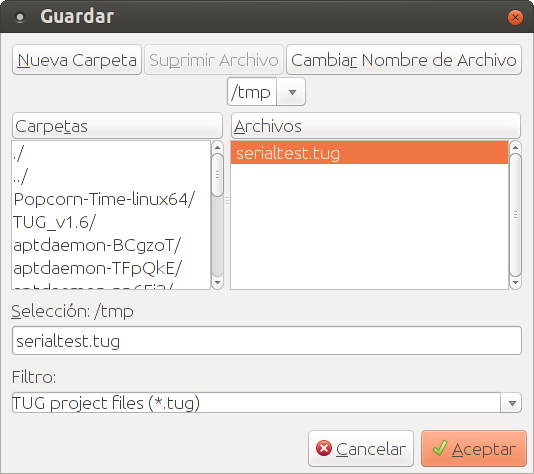
\includegraphics[width=.7\textwidth]{images/tug_save2.png}
\vspace{3ex}



\end{enumerate}
\newpage




%%% Local variables:
%%% mode: latex
%%% TeX-master: "README.tex"
%%% ispell-local-dictionary: "american"
%%% coding: utf-8
%%% fill-column: 75
%%% TeX-parse-self: t
%%% TeX-auto-save: t
%%% End:


\subsection{Test Project Generation}

Creating a project to test a Qt-based GUI is really easy by using TUG
Wizard. Please, follow the steps described in the following.

%\setcounter{enumi}{4}
\begin{enumerate}
%
%%% Select panel file
%%
\item {\bf Step 1: Select a panel.}\\
%
  Panel is the window to test. \\Click \field{1.1 Select} to select a Qt
  *.ui file.  \field{Class name} will be auto-filled based on the
  panel name found in the selected file. Please, check it.\\
%
  A test project can be also generated without a *.ui file. For this,
  select \field{There is no panel file to test} and fill \field{Class name}
  manually with a name for the panel.\\
%
  Within a Qt GUI, widgets can be referenced in many different ways (e.g.,
  by using a private implementation). By default, widgets are referenced
  using {\tt ui->}. It can be changed selecting \field{Referenced as} and
  filling this field.\\
%
  After this change, a new include could be needed. If so, select
  \field{Add this include} and click \field{1.2 Select} to select a file to
  include.\\
%
  Click \field{Next Step} at the bottom of the wizard.

\vspace{3ex}
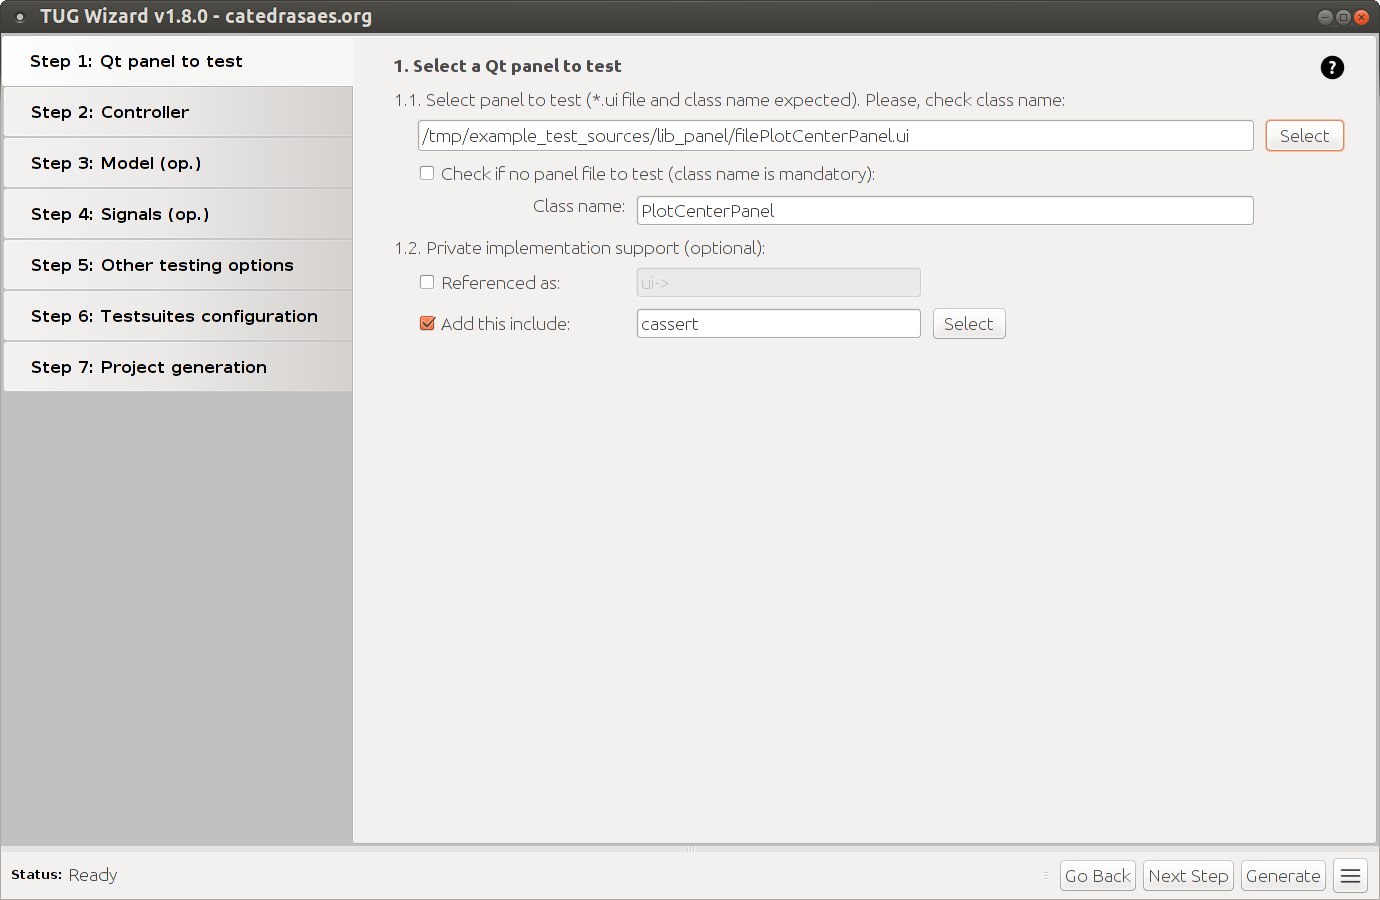
\includegraphics[width=.95\textwidth]{images/tug021.png}
\vspace{3ex}
\newpage
%
%%% 
%%
\item {\bf Step 2: Select Gateway class.}\\
%
  Gateway class (GW) is the class implementing communication with the
  manager (M).\\ 
%
  Click \field{2.1 Select} to choose the library containing the GW
  class. \\
% 
  Click \field{2.2 Select} to select the file defining the GW
  class. \field{Class name} will be auto-filled based on the class name
  found in the selected file. Please, check it. \\
% 
  Click \field{2.3 Select} to select the directory in which GW library is
  built. It is needed if coverage analysis is enabled.\\
%
  In \field{2.4} you can add additional dependencies for the GW
  library. There are some buttons to help you adding dependencies:
  \field{Add dynamic library} and \field{Add includes directory} include
        {\tt qmake} tags; \field{Add file} and \field{Add directory} can be
        used to add new paths. \\
%
  Click \field{Next Step} at the bottom of the wizard.

\vspace{3ex}
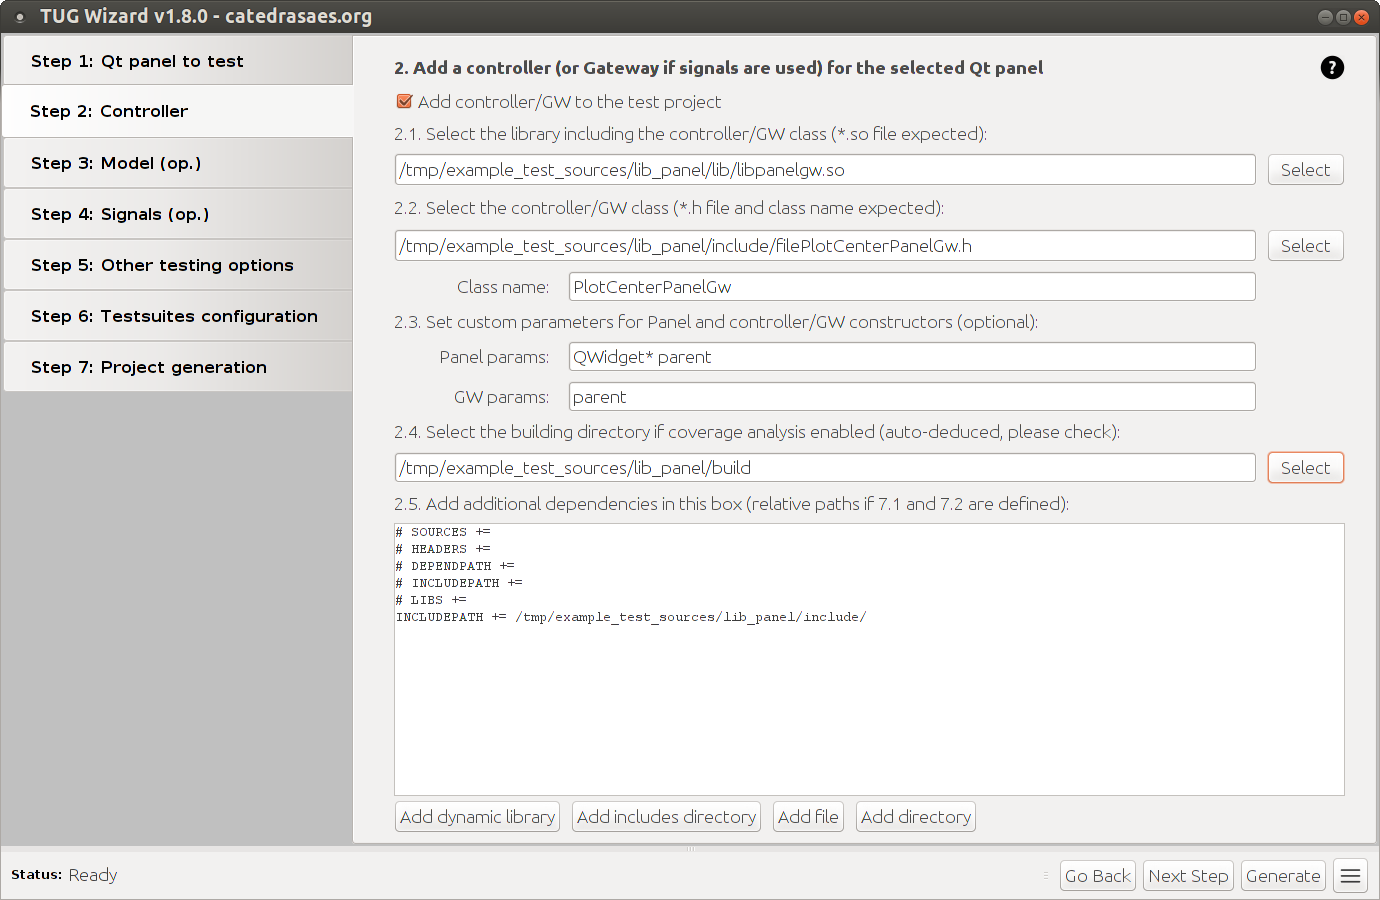
\includegraphics[width=.95\textwidth]{images/tug022.png}
\vspace{3ex}
\newpage
%
%%% 
%%
\item {\bf Step 3: Select a Manager/model (optional).}\\
%
  You can select a manager class (M) with which the panel is connected.\\
%
  Check \field{Include a manager into the testsuites} to enable this
  option. \\
%
  Click \field{3.1 Select} to choose the library containing the M class.\\
%
  Click \field{3.2 Select} to select the file defining the M
  class. \field{Class name} will be auto-filled based on the class name
  found in the selected file. Please, check it.\\
% 
  Click \field{3.3 Select} to select the directory in which M library is
  built. It is needed if coverage analysis is enabled.\\
%
  In \field{3.4} you can add additional dependencies for the M library.\\
%
  Click \field{Next Step} at the bottom of the wizard.

\vspace{3ex}
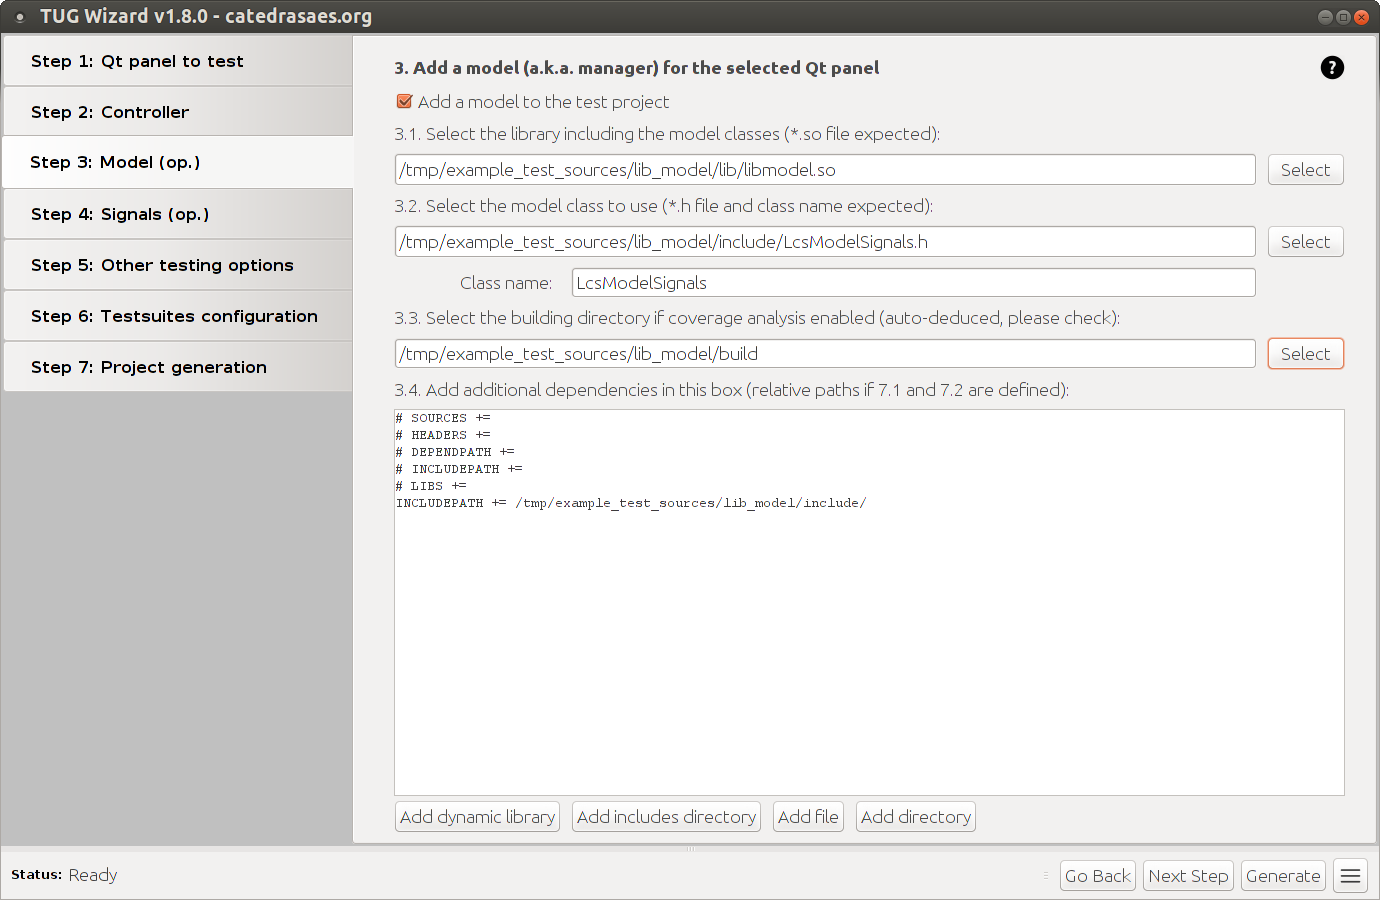
\includegraphics[width=.95\textwidth]{images/tug023.png}
\vspace{3ex}
\newpage
%
%%% 
%%
\item {\bf Step 4: Select a Signals class (optional).}\\
%
  You can select a class including those signals (S) used for the
  communication between GW and M.\\
%
  Check \field{Include a signals class into the testsuites} to enable this
  option.\\
%
  Click \field{4.1 Select} to choose the library containing the S class.\\
%
  Click \field{4.2 Select} to select the file defining the S
  class. \field{Class name} will be auto-filled based on the class name
  found in the selected file. Please, check it. \\
% 
  Click \field{4.3 Select} to select the directory in which S library is
  built. It is needed if coverage analysis is enabled.\\
%
  In \field{4.4} you can select if the signals used are based on {\tt
    Boost} or on {\tt Libsig}. You can select {\tt None} to add it
  manually. \field{Check/edit config file} can be used to check and edit
  the dependencies to be incorporated into the test project. \field{Back to
    default config} can be used to go back to default configuration of such
  dependencies. \\
%
  In \field{4.5} you can add additional dependencies for the S library.\\
%
  Click \field{Next Step} at the bottom of the wizard.

\vspace{3ex}
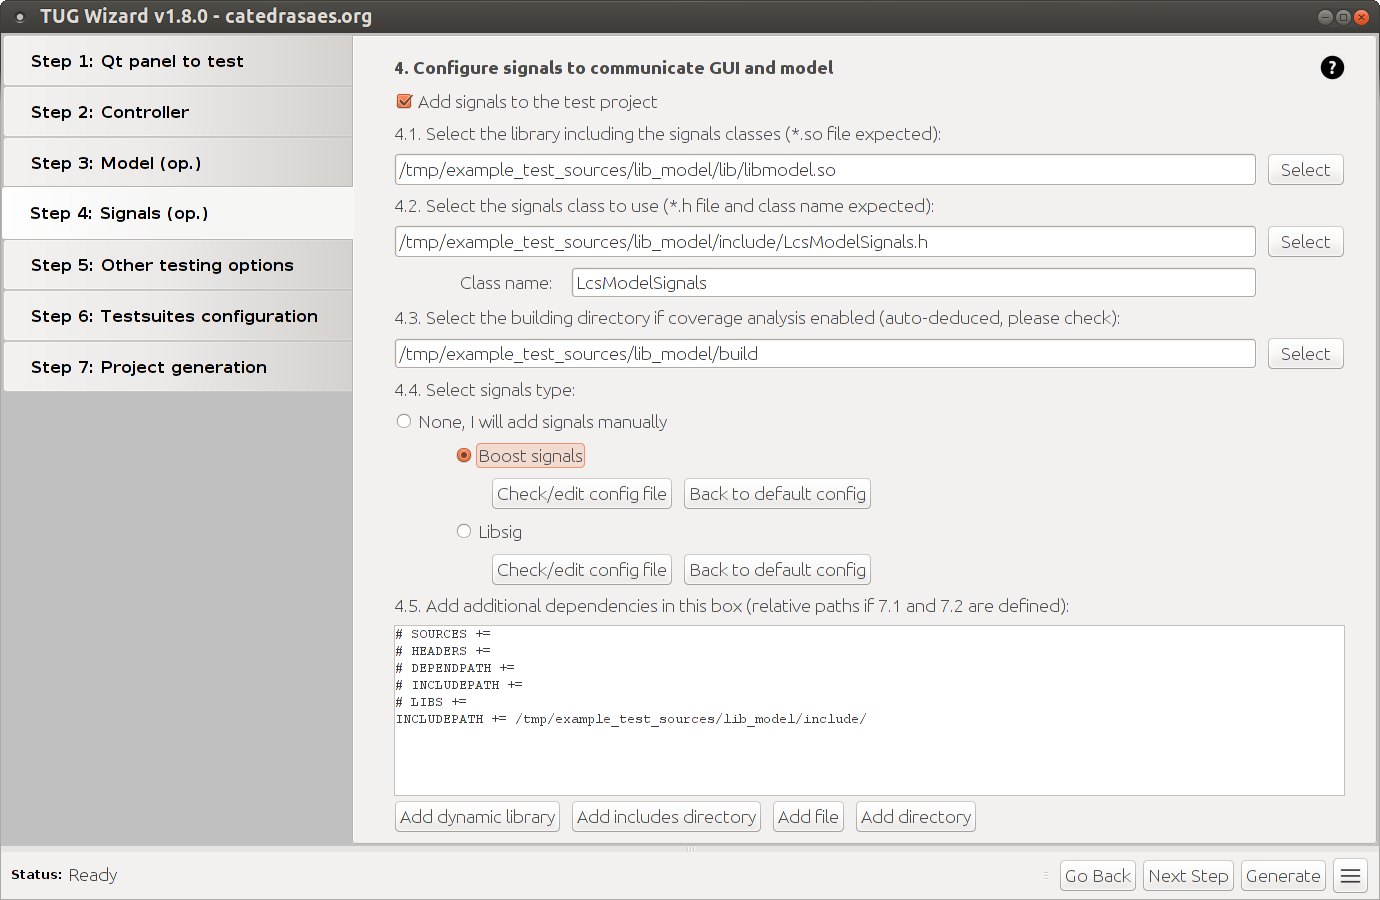
\includegraphics[width=.95\textwidth]{images/tug024.png}
\vspace{3ex}
\newpage
%
%%% 
%%
\item {\bf Step 5: Select other options for the test project.}\\
%
  In this step we can choose and configure options like coverage and
  profiling analysis, as well as add additional dependencies to the
  project.  In this step we can also check the includes for {\bf TUGLib},
  the library running under test projects generated by TUG Wizard.  \\
%
  Check \field{GCov enabled} to enable coverage analysis. \\
%
  Check \field{GProf enabled} to enable profiling. \\
%
  Check \field{Qwt enabled} to enable support for Qwt widgets. \\
%
  \field{Check/edit config file} can be used to check and edit the
  dependencies to be incorporated into the test project for each
  option. \field{Back to default config} can be used to go back to default
  configuration of such dependencies. \\
%
  In \field{5.4} you can add additional dependencies to the project. \\
%
  In \field{5.5} you can check, edit, and restore dependencies related to
  {\bf TUGLib} library.\\
%
  Click \field{Next Step} at the bottom of the wizard.

\vspace{3ex}
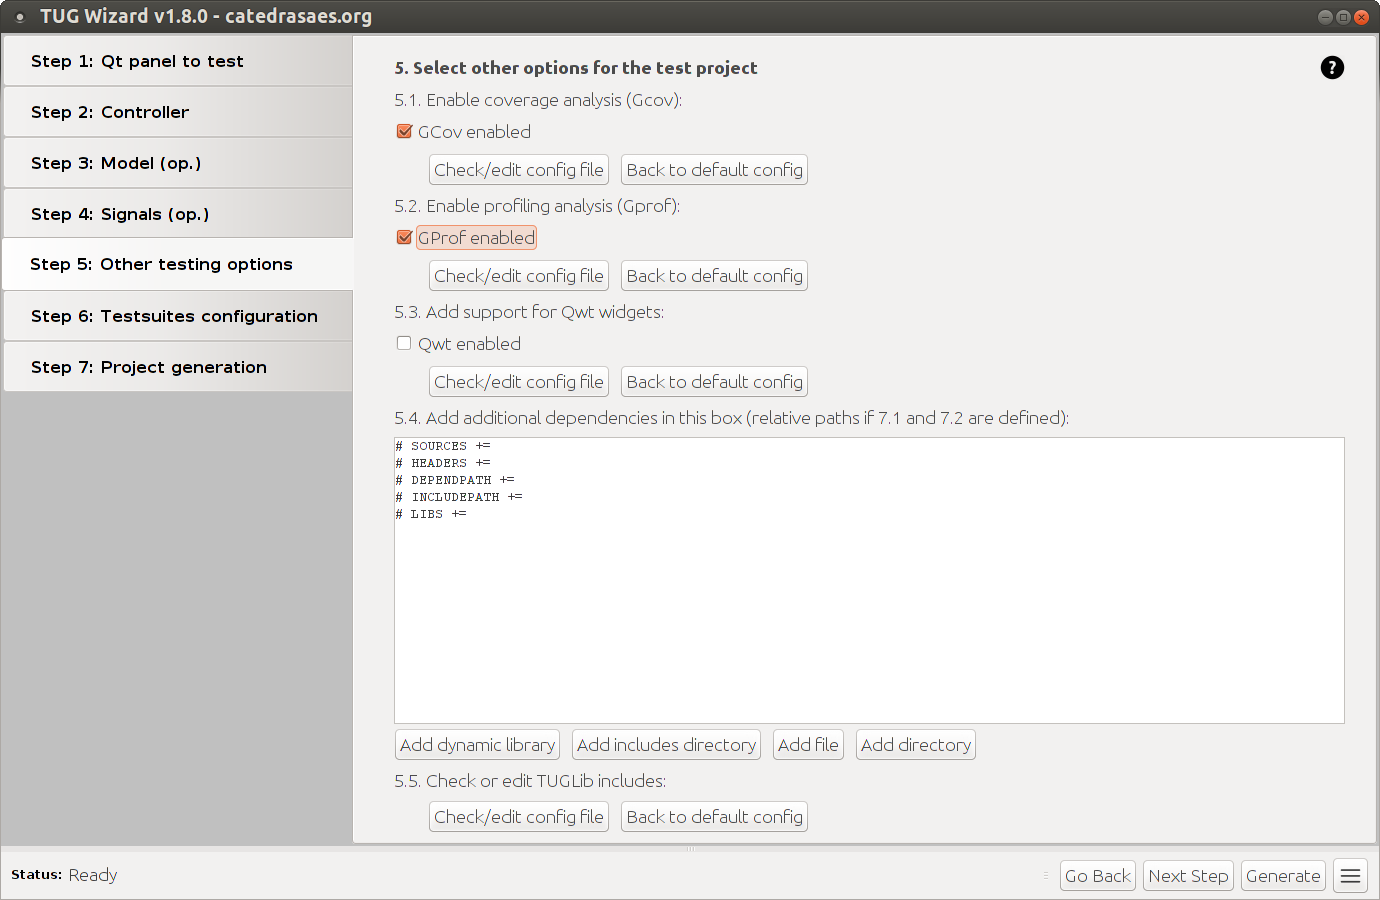
\includegraphics[width=.95\textwidth]{images/tug025.png}
\vspace{3ex}
\newpage
%
%%% 
%%
\item {\bf Step 6: Configure a testsuites structure (recommended).}\\
%
  In this step we can create the structure of a test project. As a result
  after the generation process, a set of testsuites will be auto-generated
  according to the test project configured in this step.\\
%
  Check \field{Generate test suites} to enable this option.  A
  pre-configured test project is provided as starting point. A test project
  is composed of a base testsuite (often used to configure and clean the
  test scenario) and a set of child testsuites that include some extra
  configuration (if needed) and the tests to be executed.  We can modify
  this test project as follows.\\
%
  Click \field{Add Test} to add a new test to a testsuite. Please,
  note that every testsuite (except base testsuite) must include, at
  least, one test.\\
%
  Click \field{Add Testsuite} to add a new child testsuite to a parent
  testsuite. Please, note that only level-2 testsuites are allowed
  (level-0 is base testsuite).\\
%
  Click \field{Delete Item} to delete selected item (either a test or
  a testsuite).\\
%
  Once the test project is created, click \field{Next Step} at the
  bottom of the wizard.\\
%
  \textcolor{red}{TUG Wizard implements {\bf roundtrip} between different
    versions of a test project. If a project is generated in the same
    directory it was generated before, then the code of old tests will
    be kept in the new version if they still exist.}

\vspace{3ex}
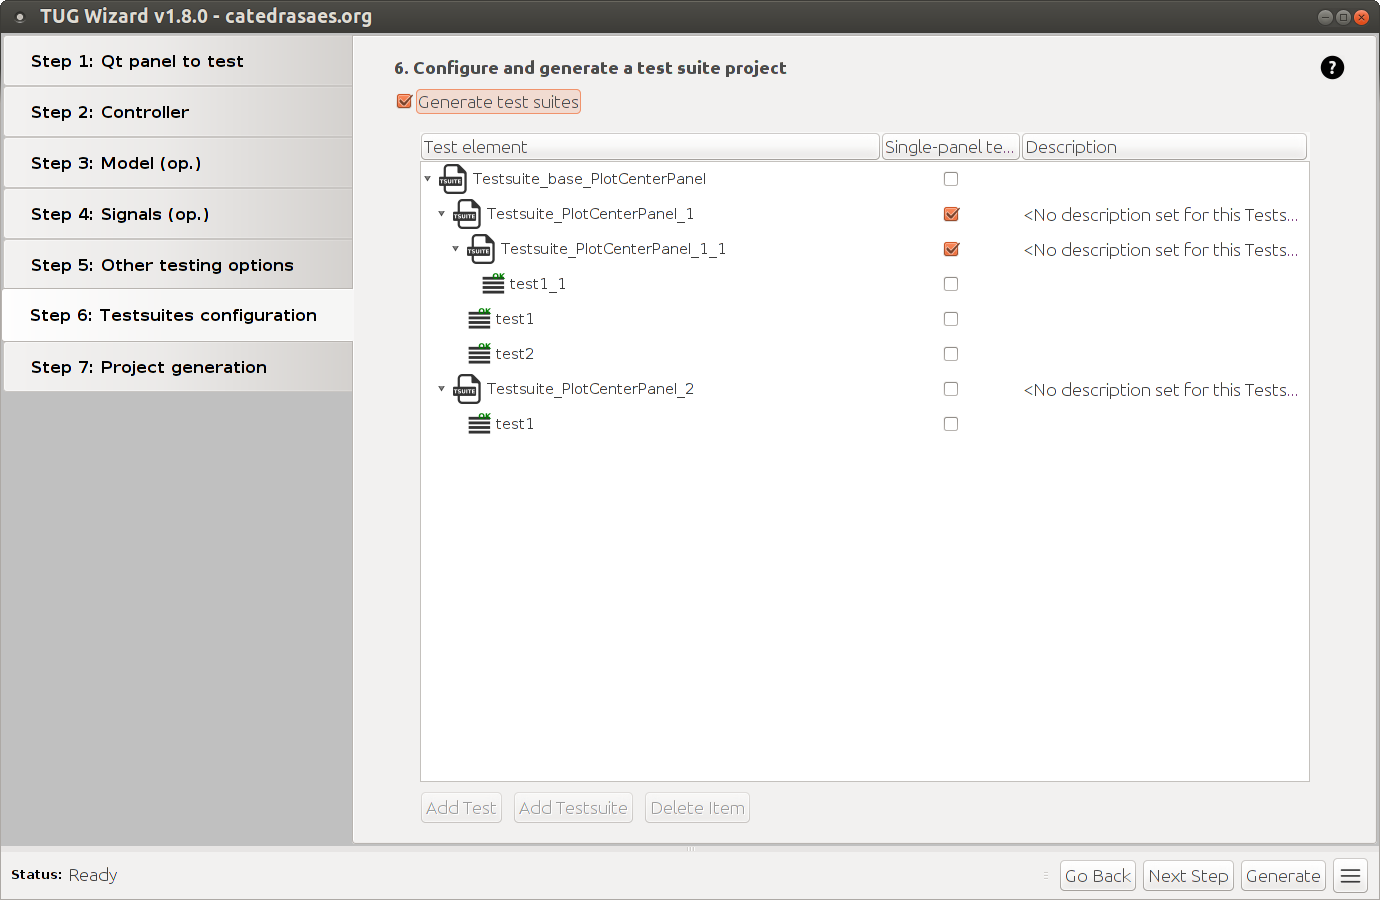
\includegraphics[width=.95\textwidth]{images/tug026.png}
\vspace{3ex}
\newpage
%
%%% 
%%
\item {\bf Step 7: Name the project and select a destination.}\\
%
  In \field{7.1} we have to add a name for our project. This name will be
  used to create a folder into which generate the project. It will be also
  used to identify the project within the output report.\\
%
  Click \field{7.2 Select} to select a directory into which generate the
  test project. Once selected, the label below this field will show the
  final destination of the test project.\\
%
  Click \field{Generate} at the bottom of the wizard to start the
  generation process. A console will appear showing generation process and
  result.

\vspace{3ex}
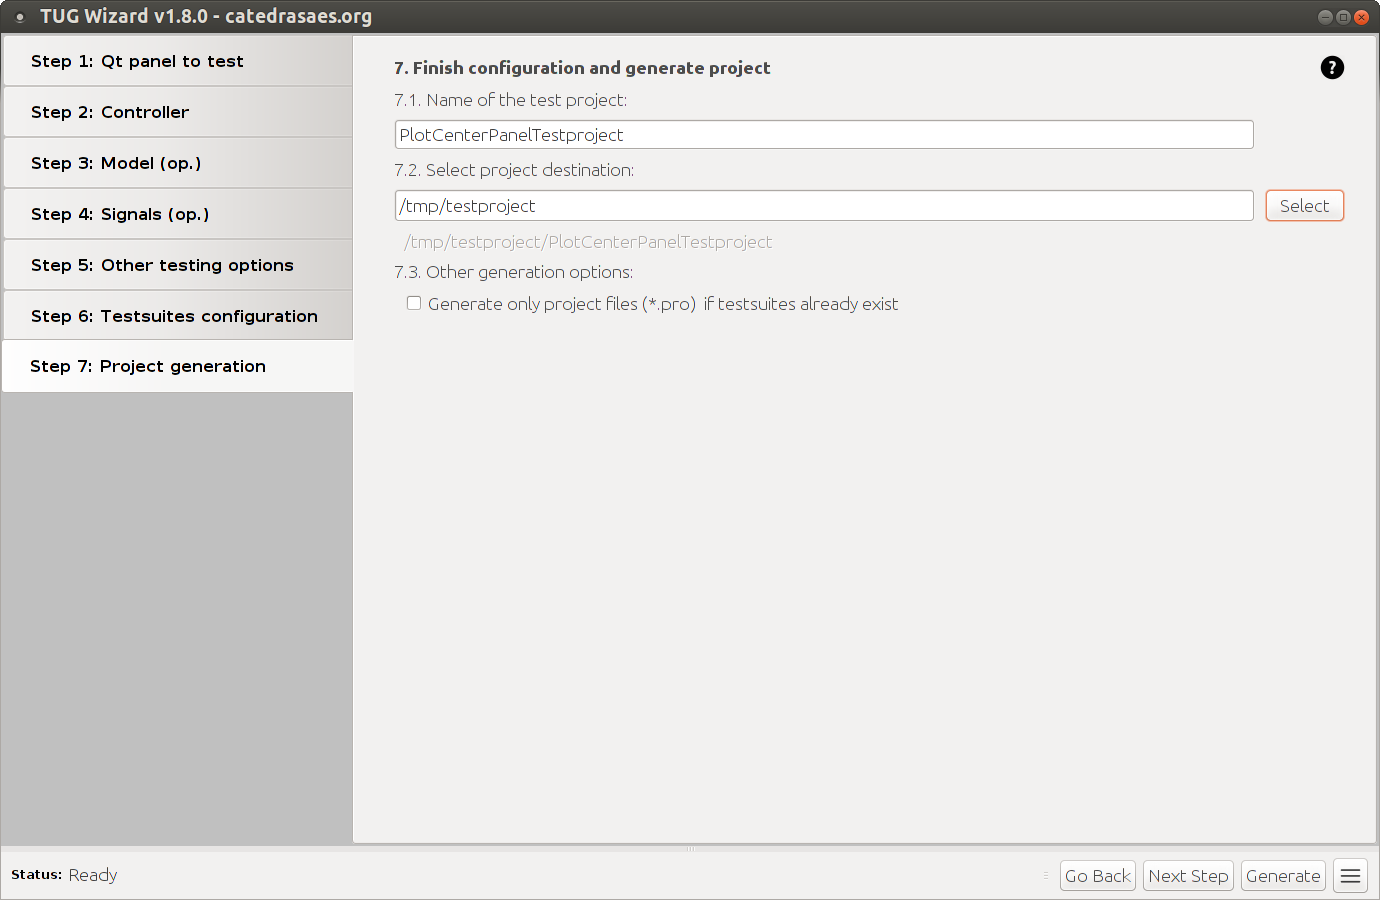
\includegraphics[width=.95\textwidth]{images/tug027.png}
\vspace{3ex}
%\newpage

%
%%% 
%%
\item {\bf Step 8: Exit the wizard.}\\
%
  Click 
\includegraphics[width=.05\textwidth]{images/menu_icon.png}
  to deploy the pop-up menu and select \field{Exit}.\\

\vspace{1ex}
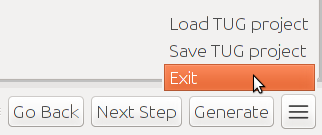
\includegraphics[width=.5\textwidth]{images/tug_exit.png}
\vspace{3ex}
\end{enumerate}
\newpage



%%% Local variables:
%%% mode: latex
%%% TeX-master: "README.tex"
%%% ispell-local-dictionary: "american"
%%% coding: utf-8
%%% fill-column: 75
%%% TeX-parse-self: t
%%% TeX-auto-save: t
%%% End:



\subsection{Test Project Compilation and Execution}

Once we have generated a test project using TUG Wizard, in this
section we are going to describe how to compile and execute the
project, as well as how to check the results obtained from its
execution. This guide assumes that Qt Creator
(\url{https://qt-project.org/wiki/Category:Tools::QtCreator}) is being
used to open, compile, and deploy Qt-based projects.

%\setcounter{enumi}{4}
\begin{enumerate}

%
%%% 
%%
\item {\bf Step 0: Project structure.}\\
%
  The generated test project is composed of:
\begin{itemize}
\item a main project (represented by {\tt build\_all.pro} file in the
  figure below) that includes all test projects, and from which they
  can be compiled.

\item a folder including all test subprojects ({\tt tests} folder in
  the figure below).
\end{itemize}


\vspace{1ex}
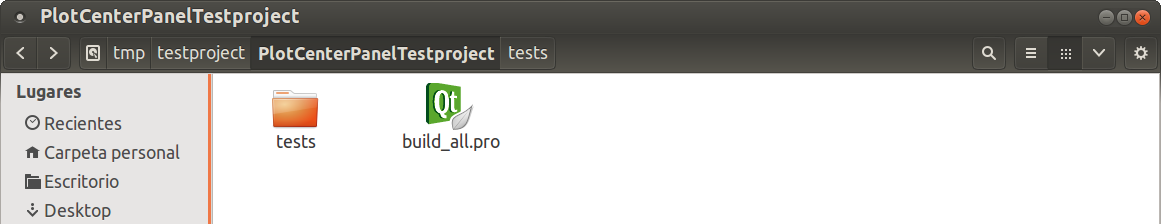
\includegraphics[width=.95\textwidth]{images/tug030a.png}
\vspace{3ex}

\newpage

Once opened the {\tt tests} folder, we can find:
\begin{itemize}

\item {\tt \_main} subproject including a class that inherits from the
  panel to test, and that includes a set of methods aimed at
  supporting the interaction with panel widgets.

\item all testsuites previously configured in TUG Wizard...

\item ...as well as the test projects from which they can be compiled
  and executed individually.
\end{itemize}

\vspace{1ex}
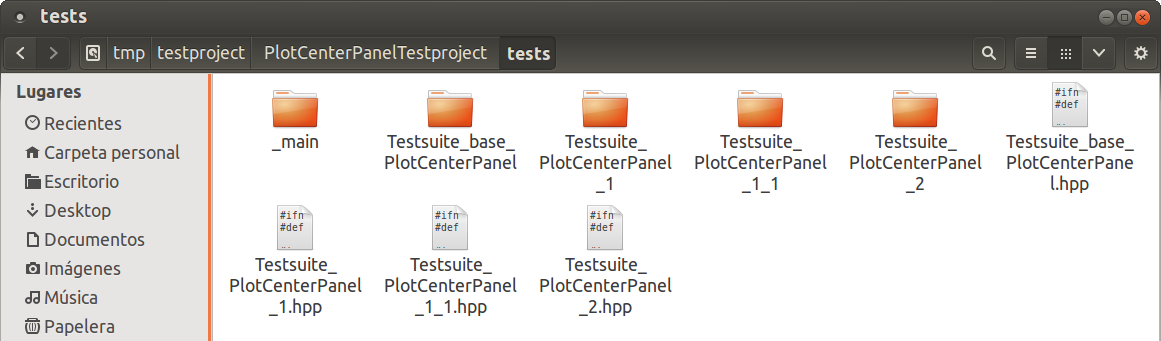
\includegraphics[width=.95\textwidth]{images/tug030b.png}
\vspace{3ex}

An snapshot of the {\_main} subproject is included below. The {\tt
  .pro} file can be opened using QtCreator to modify/compile/run the
project.

\vspace{1ex}
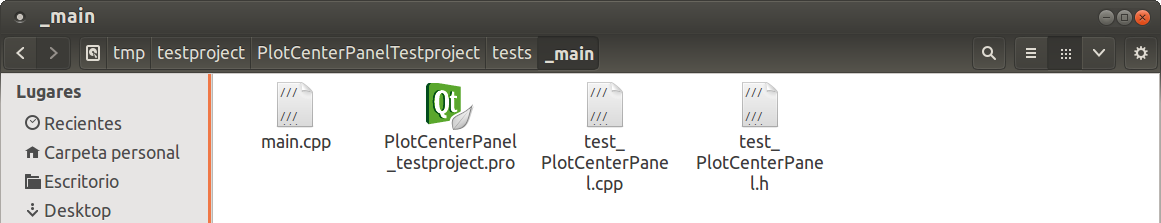
\includegraphics[width=.95\textwidth]{images/tug030c.png}
\vspace{3ex}

An snapshot of a testsuite subproject is included below.

\vspace{1ex}
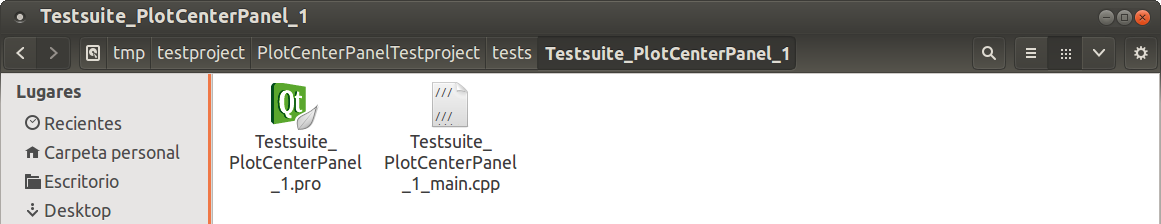
\includegraphics[width=.95\textwidth]{images/tug030d.png}
\vspace{3ex}

\newpage

%
%%% 
%%
\item {\bf Step 1: Open project.}\\
%
  Go to project folder. \\Double click
  {\tt build\_all.pro} file to open project in Qt Creator.


\vspace{1ex}
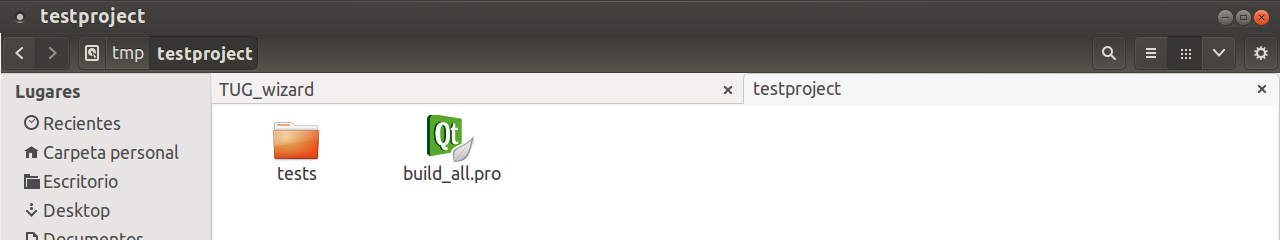
\includegraphics[width=.95\textwidth]{images/tug031.png}
\vspace{3ex}

%
%%% 
%%
\item {\bf Step 2: Configure project (i).}\\
%
  Once in Qt Creator, in
  \field{Configure Project} window, check only \field{Debug} version
  and click \field{Configure Project}.


\vspace{1ex}
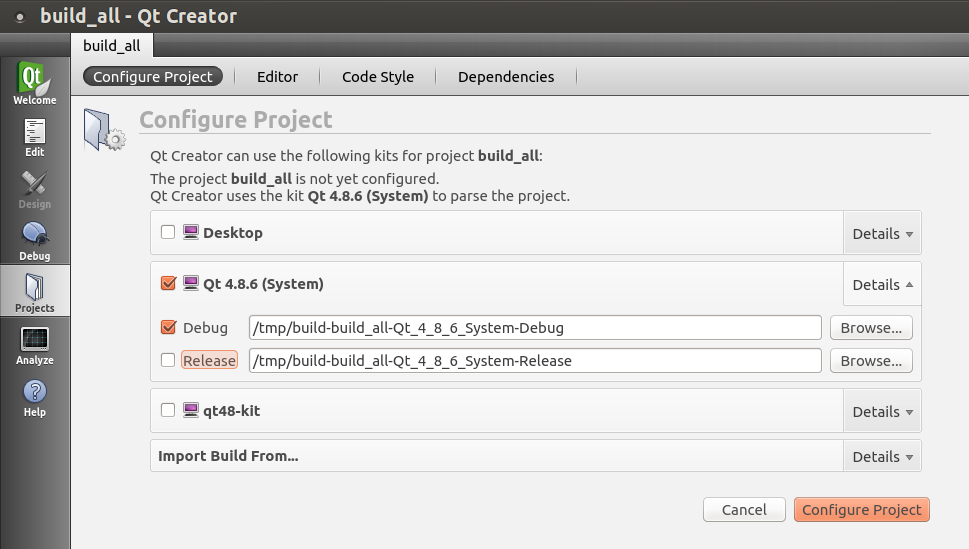
\includegraphics[width=.95\textwidth]{images/tug032.png}
\vspace{3ex}
\newpage

%
%%% 
%%
\item {\bf Step 3: Configure project (ii).}\\
%
  Go to \field{Projects}
  section in the tools bar at left. \\Uncheck \field{Shadow Build}.


\vspace{1ex}
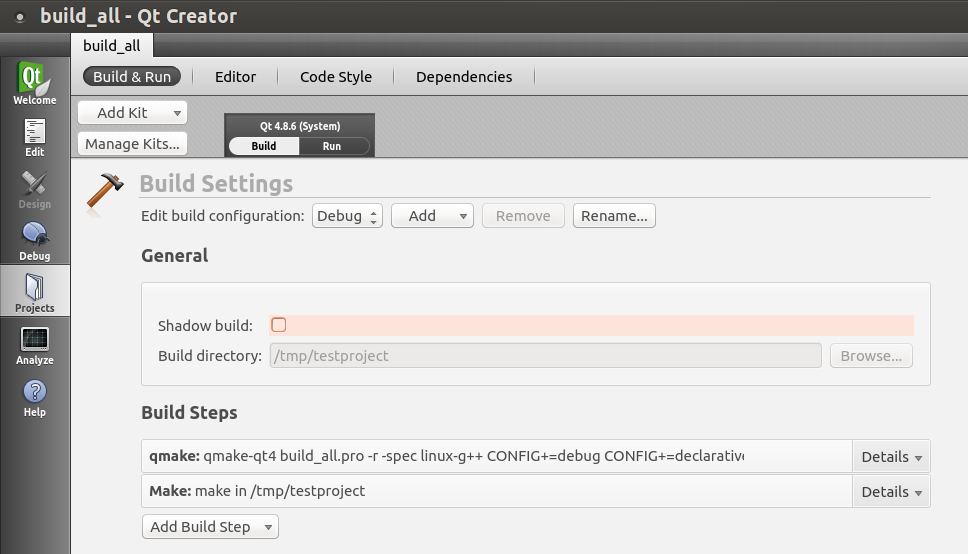
\includegraphics[width=.95\textwidth]{images/tug033.png}
\vspace{3ex}

%
%%% 
%%
\item {\bf Step 4: Project compilation.}\\
%
  Go to \field{Edit}
  section in the tools bar at left. \\Right click on
  \field{build\_all.pro} at the top of the projects list and then
  click \field{Rebuild}.

\vspace{1ex}
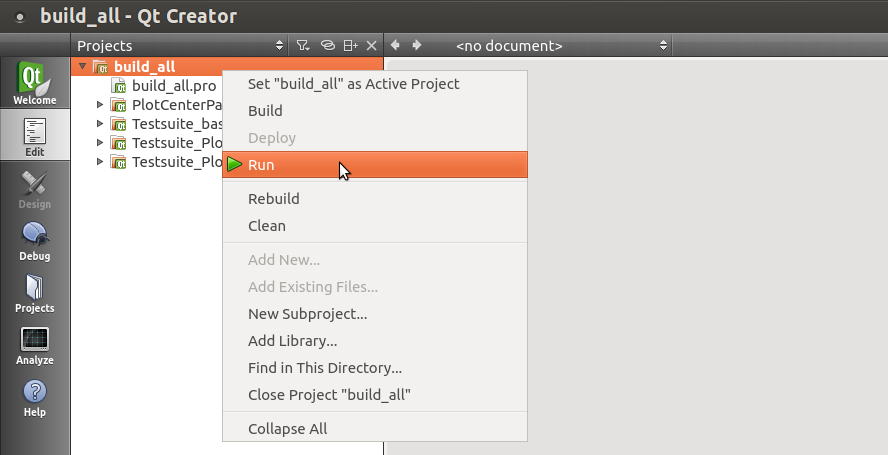
\includegraphics[width=.95\textwidth]{images/tug034.png}
\vspace{3ex}
\newpage

%
%%% 
%%
\item {\bf Step 5: Project execution.}\\
%
  Go to main project (it is
  placed the first in the project list), right click on it and then
  click \field{Run}.

\vspace{1ex}
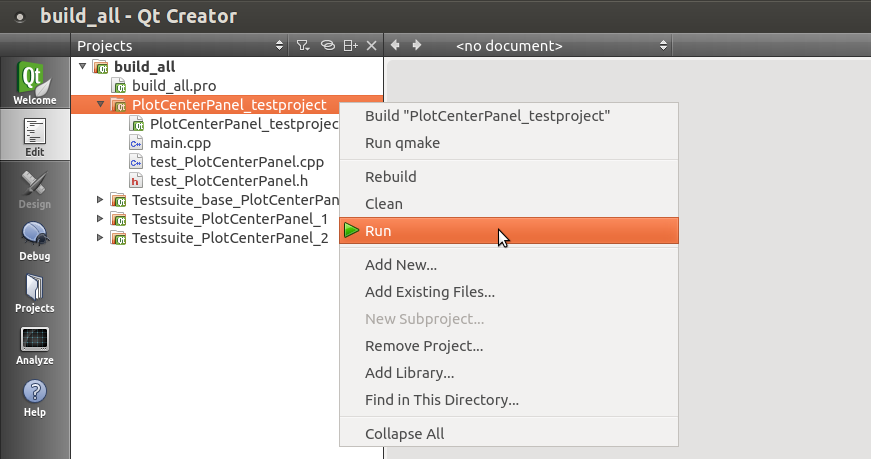
\includegraphics[width=.95\textwidth]{images/tug035.png}
\vspace{3ex}

%
%%% 
%%
\item {\bf Step 6: Check project output.}\\
%
  In the project folder, go to
  {\tt out} folder and open {\tt output.xml.html} file to see a
  summary of execution results.

\vspace{1ex}
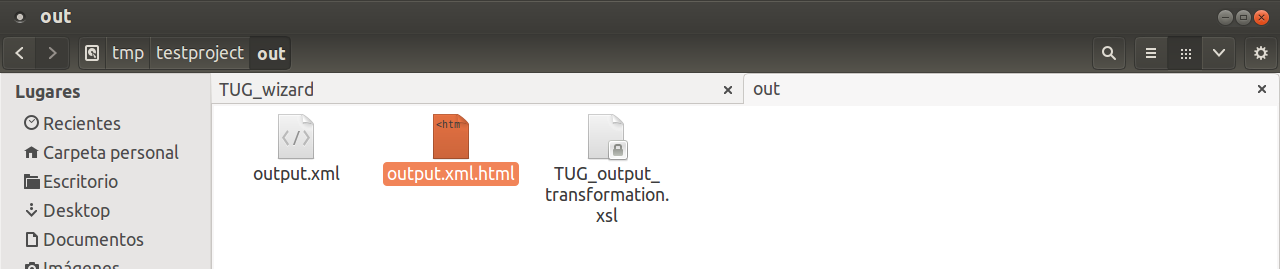
\includegraphics[width=.95\textwidth]{images/tug036.png}
\vspace{3ex}


\end{enumerate}



%%% Local variables:
%%% mode: latex
%%% TeX-master: "README.tex"
%%% ispell-local-dictionary: "american"
%%% coding: utf-8
%%% fill-column: 75
%%% TeX-parse-self: t
%%% TeX-auto-save: t
%%% End:



%%% Local variables:
%%% mode: latex
%%% TeX-master: "README.tex"
%%% ispell-local-dictionary: "american"
%%% coding: utf-8
%%% fill-column: 75
%%% TeX-parse-self: t
%%% TeX-auto-save: t
%%% End:


\section{TUG Base Library}
\label{sec:tuglib}


\subsection{Library Design}

TUG Base Library is the supporting library used by test projects
generated using TUG Wizard. Its architecture design is depicted in the
figure below. 

\vspace{2ex}
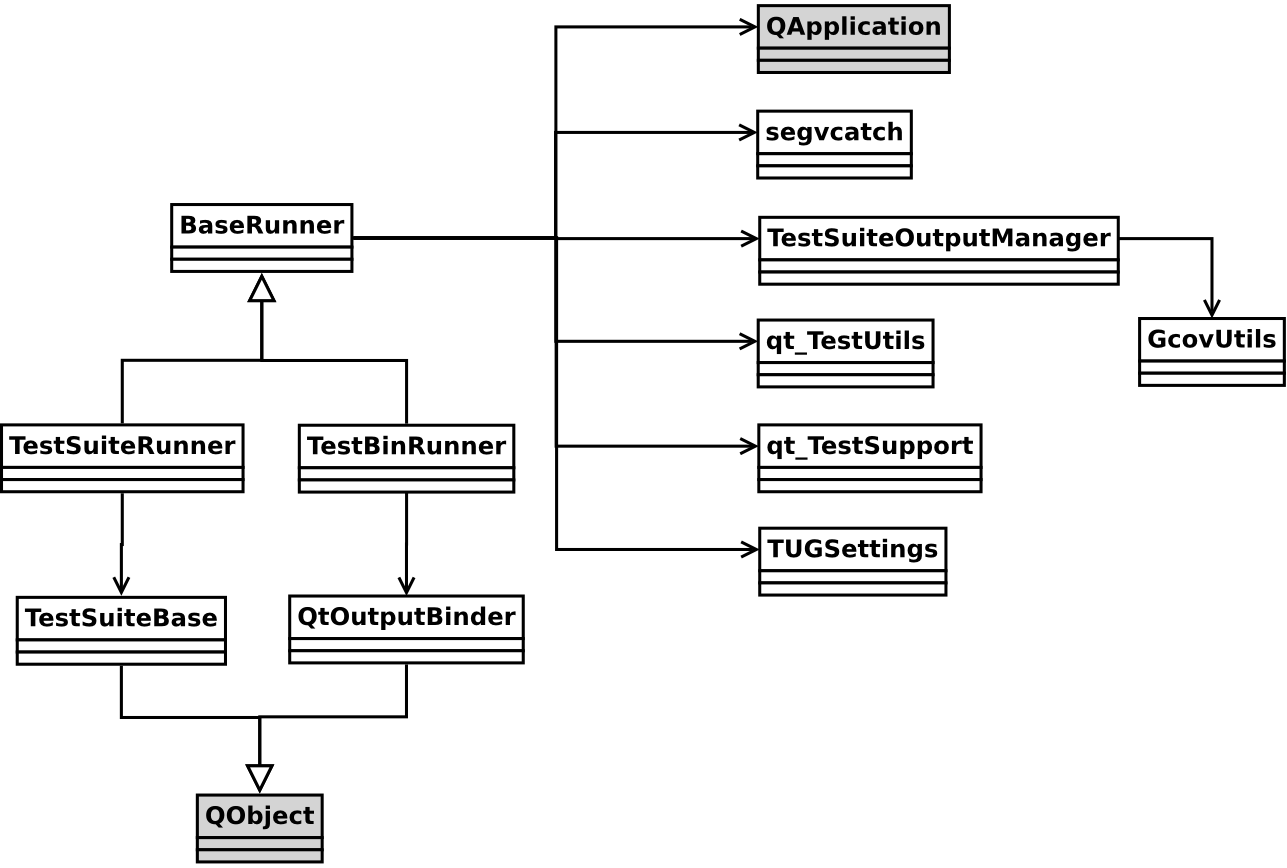
\includegraphics[width=.99\textwidth]{images/diag/tug_lib_classdiag.png}
\vspace{2ex}

Main elements of this architecture are described in the following:
\begin{itemize}
\item {\tt TestSuiteBase}
\item {\tt BaseRunner}
\item {\tt TestSuiteRunner}
\item {\tt TestBinRunner}
\item {\tt qt\_TestUtils}
\item {\tt qt\_TestSupport}
\end{itemize}

\newpage

%%%
%%%
\field{TestSuiteBase} is the base class for any testsuite. It
implements the basic functionality of a test suite, and includes also
some virtual methods to be implemented in subclasses. It extends {\tt
  QObject} class to be integrated in Qt Test framework.


The code snippet below shows how new testsuites have to be defined:

\begin{lstlisting}
#include "TestSuiteBase.h"

class Testsuite_base_Panel : public TestSuiteBase {

    Q_OBJECT /// Our test suite has to execute Q_OBJECT macros

    (...)
\end{lstlisting}

Testsuites based on {\tt TestSuiteBase} can be created as object and
executed standalone by using the following methods:

\begin{lstlisting}
//
static int 
 launch_standalone (TestSuiteBase* tsb, int argc=0, char *argv[]=0);
//
static int 
 launch (TestSuiteBase* tsb, QApplication* app);
//
static int 
 launch (TestSuiteBase* tsb, QApplication* app, int argc,char** argv);
\end{lstlisting}


One or more {\tt TestSuiteBase} objects can be also be launched
sequentially using {\tt TestSuiteRunner}, as described below.


\newpage

%%%
%%%
\field{BaseRunner} includes the basic functionality to run tests. Tests
can be run from a testsuite class file using {\tt TestSuiteRunner}, or
from a testsuite binary using {\tt TestBinRunner}. 
%
The former has the advantage that no previously compiled binaries are
needed, and that all tests are encapsulated into a single binary file.
%
The latter has the advantage that tests are executed as independent
binary files, allowing thus to handle segmentation faults. This is the
option used in TUG Wizard.

All relevant methods and options supported by {\tt BaseRunner} are
described in the following:
\begin{itemize}
%
\item {\tt BaseRunner\& add\_timestamp\_to\_output\_filename()}: adds a
  timestamp to the name of the generated output files.
%
\item {\tt BaseRunner\& coverage\_on\_dir(const std::string\& dir)}:
  includes directory {\tt dir} into coverage analysis.
%
\item {\tt BaseRunner\& coverage\_on\_file(const std::string\&
  filepath)}: includes file {\tt filepath} into coverage analysis.
%
\item {\tt BaseRunner\& output\_***()}: selects output level between
  {\tt silent}, {\tt verbose}, {\tt extended} or {\tt all}.
%
\item {\tt BaseRunner\& pause\_between(int ms)}: sets idle time
  between the execution of a test and the following one.
%
\item {\tt BaseRunner\& project\_name(const std::string name)}: sets a
  name for the test project. This name is used if a report is
  generated.
%
\item {\tt void reset()}: resets runner values.
%
\item {\tt int run()}: run the tests previously added to the runner.
%
\end{itemize}


\newpage

%%%
%%%
\field{TestSuiteRunner} can be used to run testsuite files. It
provides the method {\tt add\_testsuite()} to add a new testsuite
object to the runner. Testsuites objects are run sequentially. If a
test causes segmentation fault or another similar error, next text
will not be executed.

The code snippet below shows how {\tt TestSuiteRunner} has to be
defined and properly configured. In the example, a project name is
given, output is configured, and coverage targets are set. A new
testsuite object is created and added to the runner. Finally, the
tests are run. 

\begin{lstlisting}
#include <TestSuiteRunner.h>
#include "testsuite_Panel_1.hpp"

int main(int argc, char *argv[])
{
    /// 1. create a TestSuiteRunner and configure...
    TestSuiteRunner trunner(argc,argv);
    trunner.project_name("PanelTestproject");

    // output options
    trunner.output_verbose();

    // coverage options
    trunner.coverage_on_file("/adir/afile.cpp")
           .coverage_on_dir("/adir/");

    /// 2. add testsuites to the runner
    testsuite_Panel_1 ts1;
    trunner.add_testsuite(&ts1);

    /// 3. run testsuites
    return trunner.pause_between(1000).run_testsuites();
}
\end{lstlisting}



\newpage


%%%
%%%
\field{TestBinRunner} can be used to run testsuite binaries (i.e.,
testsuite projects already compiled). It provides the method {\tt
  add\_testbin()} to add a new testsuite binary to the
runner. Testsuites binaries are run sequentially. If a test causes
segmentation fault or another similar error, runner tries to recover
output data and then executes next test.

The code snippet below shows how {\tt TestBinRunner} has to be defined
and properly configured. In the example, a project name is given,
output is configured, and coverage targets are set. A new testsuite
binary is added to the runner using a relative path. Finally, the
tests are run.


\begin{lstlisting}
#include <TestBinRunner.h>

int main(int argc, char *argv[])
{
    /// 1. create a test runner and configure...
    TestBinRunner trunner(argc,argv);
    trunner.project_name("PanelTestproject");

    // output options
    trunner.output_verbose();

    // coverage options
    trunner.coverage_on_file("/adir/afile.cpp")
           .coverage_on_dir("/adir/");

    /// 2. add test binaries to the runner
    trunner.add_testbin("./Testsuite_PlotCenterPanel_1_1");

    /// 3. run tests
    return trunner.pause_between(1000).run();
}
\end{lstlisting}

\vspace{2ex}


%%%
%%%
\field{qt\_TestUtils} includes a set of methods aimed at supporting the
definition of new tests (e.g., launch or repaint a panel, sleep some
milliseconds, assert values, generate random variables, simulate
segmentation faults, send data to logs, range macros, etc).\\
%
\indent \field{qt\_TestSupport} includes a set of methods to manipulate Qt GUI
widgets. These methods try to simulate user interaction.\\
%
Relevant methods in these classes are further described in next subsection.



\newpage




%%% Local variables:
%%% mode: latex
%%% TeX-master: "README.tex"
%%% ispell-local-dictionary: "american"
%%% coding: utf-8
%%% fill-column: 75
%%% TeX-parse-self: t
%%% TeX-auto-save: t
%%% End:


\subsection{Library Utils for Writing Tests}

As said above, {\tt qt\_TestUtils} includes a set of methods aimed at
supporting the definition of new tests. These methods can be accessed
through the namespace {\tt tug::}.
%
Some of these methods are described next.

\vspace{1ex}

Launch and destroy panels:
%
\begin{lstlisting}
// launches a panel/window object
void panel_launch(QWidget* panel)
void panel_launch(QWidget& panel)

// deletes a panel/window object
void panel_destroy(QWidget* panel)
void panel_destroy(QWidget& panel)
\end{lstlisting}

\begin{lstlisting}
Example:
----------------------------------------------------------------------
test_panel panel;
tug::panel_launch(panel);
\end{lstlisting}


Assertions:
%
\begin{lstlisting}
// checks a boolean expression
void assert(bool expr)

// checks a boolean expression and displays 'msg' if error
void assert_msg(bool expr, const char* msg)

// prints a warning message in a test
void warning(const char* msg)

// simulates an error in a test
void fail(const char* msg)
\end{lstlisting}

\begin{lstlisting}
Example:
----------------------------------------------------------------------
tug::assert(1 == true);
tug::assert_msg(1 == false,``This will never be true'');
tug::warning(``This is a warning message'');
tug::fail(``Simulating a failure'');
\end{lstlisting}


Update/repaint panels:
%
\begin{lstlisting}
// repaints a panel
void panel_repaint(QWidget* panel)
void panel_repaint(QWidget& panel)

// hides and shows a panel. It forces repaint and update.
void panel_blink(QWidget* panel)
void panel_blink(QWidget& panel)
\end{lstlisting}

\begin{lstlisting}
Example:
----------------------------------------------------------------------
test_panel panel; tug::panel_launch(panel);
// do something here...
tug::panel_repaint(panel); //this repaints the user interface
// do something more...
tug::panel_blink(panel); //this forces a panel update
\end{lstlisting}


Sleeps:
%
\begin{lstlisting}
// sleeps 'ms' milliseconds
void sleep(int ms)

// sleeps 1 second
void sleep1()

// sleeps 2 second
void sleep2()

// sleeps 3 second
void sleep3()

// sleeps 5 second
void sleep5()
\end{lstlisting}

\begin{lstlisting}
Example:
----------------------------------------------------------------------
tug::sleep2();
\end{lstlisting}


Random values:
%
\begin{lstlisting}
// resets random numbers generator
void random_reset()

// generates a random number between 0 and 'n'
int random(int n)

// generates a random number between 'low' and 'high'
int random_in_range(int low, int high)

// generates true or false randomly
bool random_bool()
\end{lstlisting}

\begin{lstlisting}
Example:
----------------------------------------------------------------------
tug::random_reset();
panel->amethod_expecting_int(tug::random(10));
panel->amethod_expecting_percentage(tug::random(0,100));
panel->amethod_expecting_bool(tug::random_bool());
\end{lstlisting}


Simulation of segmentation faults:
%
\begin{lstlisting}
// simulates a segmentation fault
void segfault()
\end{lstlisting}

\begin{lstlisting}
Example:
----------------------------------------------------------------------
tug::segfault(); //at this point a testsuite ends its execution
\end{lstlisting}



Timers:
%
\begin{lstlisting}
/// starts timer
void timer_start()

/// returns milliseconds elapsed from last call to timer_start
long timer_elapsed_ms()
\end{lstlisting}

\begin{lstlisting}
Example:
----------------------------------------------------------------------
tug::timer_start();

tug::sleep1();
tug::log() << "timer 1: " << tug::timer_elapsed_ms();
tug::sleep2();
tug::log() << "timer 2: " << tug::timer_elapsed_ms();

tug::timer_start(); //timer reset

tug::sleep2();
tug::log() << "timer 3: " << tug::timer_elapsed_ms();
\end{lstlisting}


Ranges:
%
\begin{lstlisting}
/// ForRange
template <typename T>
class ForRange(T l, T u) 

/// ForNestedRange
template <typename T>
class ForNestedRange(T l, T u, T li, T ui)
\end{lstlisting}

\begin{lstlisting}
Example:
----------------------------------------------------------------------
tug::ForRange<double>(-10,70)
   .call<test_panel>(_panel, &test_panel::set_sbLatMin)
   .call_void<test_panel>(_panel, &test_panel::doClick_btApplyCenter)
   .repaint(_panel) //optional
   .sleep_ms(100)   //optional - default is 0
   .increment(2)    //optional - default is 1
   .run();

tug::ForNestedRange<int>(-100,100,-200,200)
   .call<test_panel>(_panel, &test_panel::set_sbLatDegrees)
   .call_inner<test_panel>(_panel, &test_panel::set_sbLongDegrees)
   .call_void<test_panel>(_panel, &test_panel::doClick_btApplyCenter)
   .repaint(_panel) //optional
   .increment(5)    //optional - default is 1
   .run();
\end{lstlisting}


Log:
%
\begin{lstlisting}
// log adds a log line to a test
void log(const char* s)
\end{lstlisting}

\begin{lstlisting}
Example:
----------------------------------------------------------------------
tug::log(``log a sentence...'');
tug::log() << ``or use it as `` << 1 << `` stream.'';
\end{lstlisting}


Macros for value ranges (out of {\tt tug::} namespace):
%
\begin{lstlisting}
// This macro repeates a code 'n' times. 
// Additionally, values from 0 to 'n-1' are generated.
// 'value' is the name of the variable to be used.
tug__REPEAT(n)

// This macro simulates an integer range between 'min' and 'max', both
// included.
// 'value' is the name of the variable to be used.
tug__INT_RANGE(min,max)

// This macro simulates an integer range between 'min' and 'max', both
// included, using 'inc' as increment.
// 'value' is the name of the variable to be used.
tug__INT_RANGE_INC(min,max,inc)

// This macro simulates a float range between 'min' and 'max', both
// included, using 'inc' as increment.
// 'value' is the name of the variable to be used.
tug__FLOAT_RANGE(min,max,inc)

// This macro executes a code 'n' iterations. 
// At each iteration 'value' holds a random value between 0 
// and 'random_limit'.
// 'value' is the name of the variable to be used.
tug__RANDOM_INT_SET(n,random_limit)

// This macro executes a code 'n' iterations.
// At each iteration 'value' holds a random value true or false.
// 'value' is the name of the variable to be used.
tug__RANDOM_BOOL_SET(n)
\end{lstlisting}









%%% Local variables:
%%% mode: latex
%%% TeX-master: "README.tex"
%%% ispell-local-dictionary: "american"
%%% coding: utf-8
%%% fill-column: 75
%%% TeX-parse-self: t
%%% TeX-auto-save: t
%%% End:


\subsection{Library Configuration}

Some options of TUG Base Library can be configured in \field{settings}
file. For changes in this file to take effect, it is needed to recompile
the library after saving it.
%
Some of the options that can be changed are briefly described in the
following.


\vspace{1ex}

Commands used to gather to coverage and profiling information:
%
\begin{lstlisting}
### gcov/lcov/gprof commands

gcov_pre_command = "gcov"
gcov_pre_options = "-p -r -n -o ##FILEPATH## ##FILEPATH##;"
gcov_post_command = ""
gcov_post_options = ""
gcov_clean_command = "rm *.gcda *.gcov;"

gprof_pre_command = "gprof"
gprof_pre_options = "-p -b ##BINNAME## gmon.out;"
gprof_post_command = ""
gprof_post_options = ""
gprof_clean_command = "rm gmon.out;"

lcov_pre_command = "lcov"
lcov_pre_options = "-z --directory ##SOURCEDIR##;"
lcov_post_command = "lcov"
lcov_post_options = "--capture --ignore-errors graph --directory ##SOURCEDIR## --output-file /tmp/coverage.info; genhtml /tmp/coverage.info --output-directory ##DESTDIR##;"
lcov_clean_command = "rm /tmp/coverage.info;"
\end{lstlisting}


Directories in which include generated artifacts:
%
\begin{lstlisting}
### main directories

# dir paths relatives to "maintest"
dir_bin = "../bin"
dir_coverage = "../coverage"
dir_output = "../out"
dir_tests = "../bin"
\end{lstlisting}


File names used during output management:
%
\begin{lstlisting}
### output file

output_style_filename = "TUG_output_transformation.xsl"
output_temp_file = "/tmp/___tug_test_output";
output_final_filename = "output.xml";
\end{lstlisting}

\newpage







%%% Local variables:
%%% mode: latex
%%% TeX-master: "README.tex"
%%% ispell-local-dictionary: "american"
%%% coding: utf-8
%%% fill-column: 75
%%% TeX-parse-self: t
%%% TeX-auto-save: t
%%% End:




%%% Local variables:
%%% mode: latex
%%% TeX-master: "README.tex"
%%% ispell-local-dictionary: "american"
%%% coding: utf-8
%%% fill-column: 75
%%% TeX-parse-self: t
%%% TeX-auto-save: t
%%% End:


\section{TUG Wizard Design and Configuration}
\label{sec:tugwizarddesignconfig}


\subsection{Wizard Design}

TUG Wizard is a wizard-like application that helps developers create and
configure test projects to test Qt based panels and their related classes.
%
Its architecture design is depicted in the figure below.

\vspace{2ex}
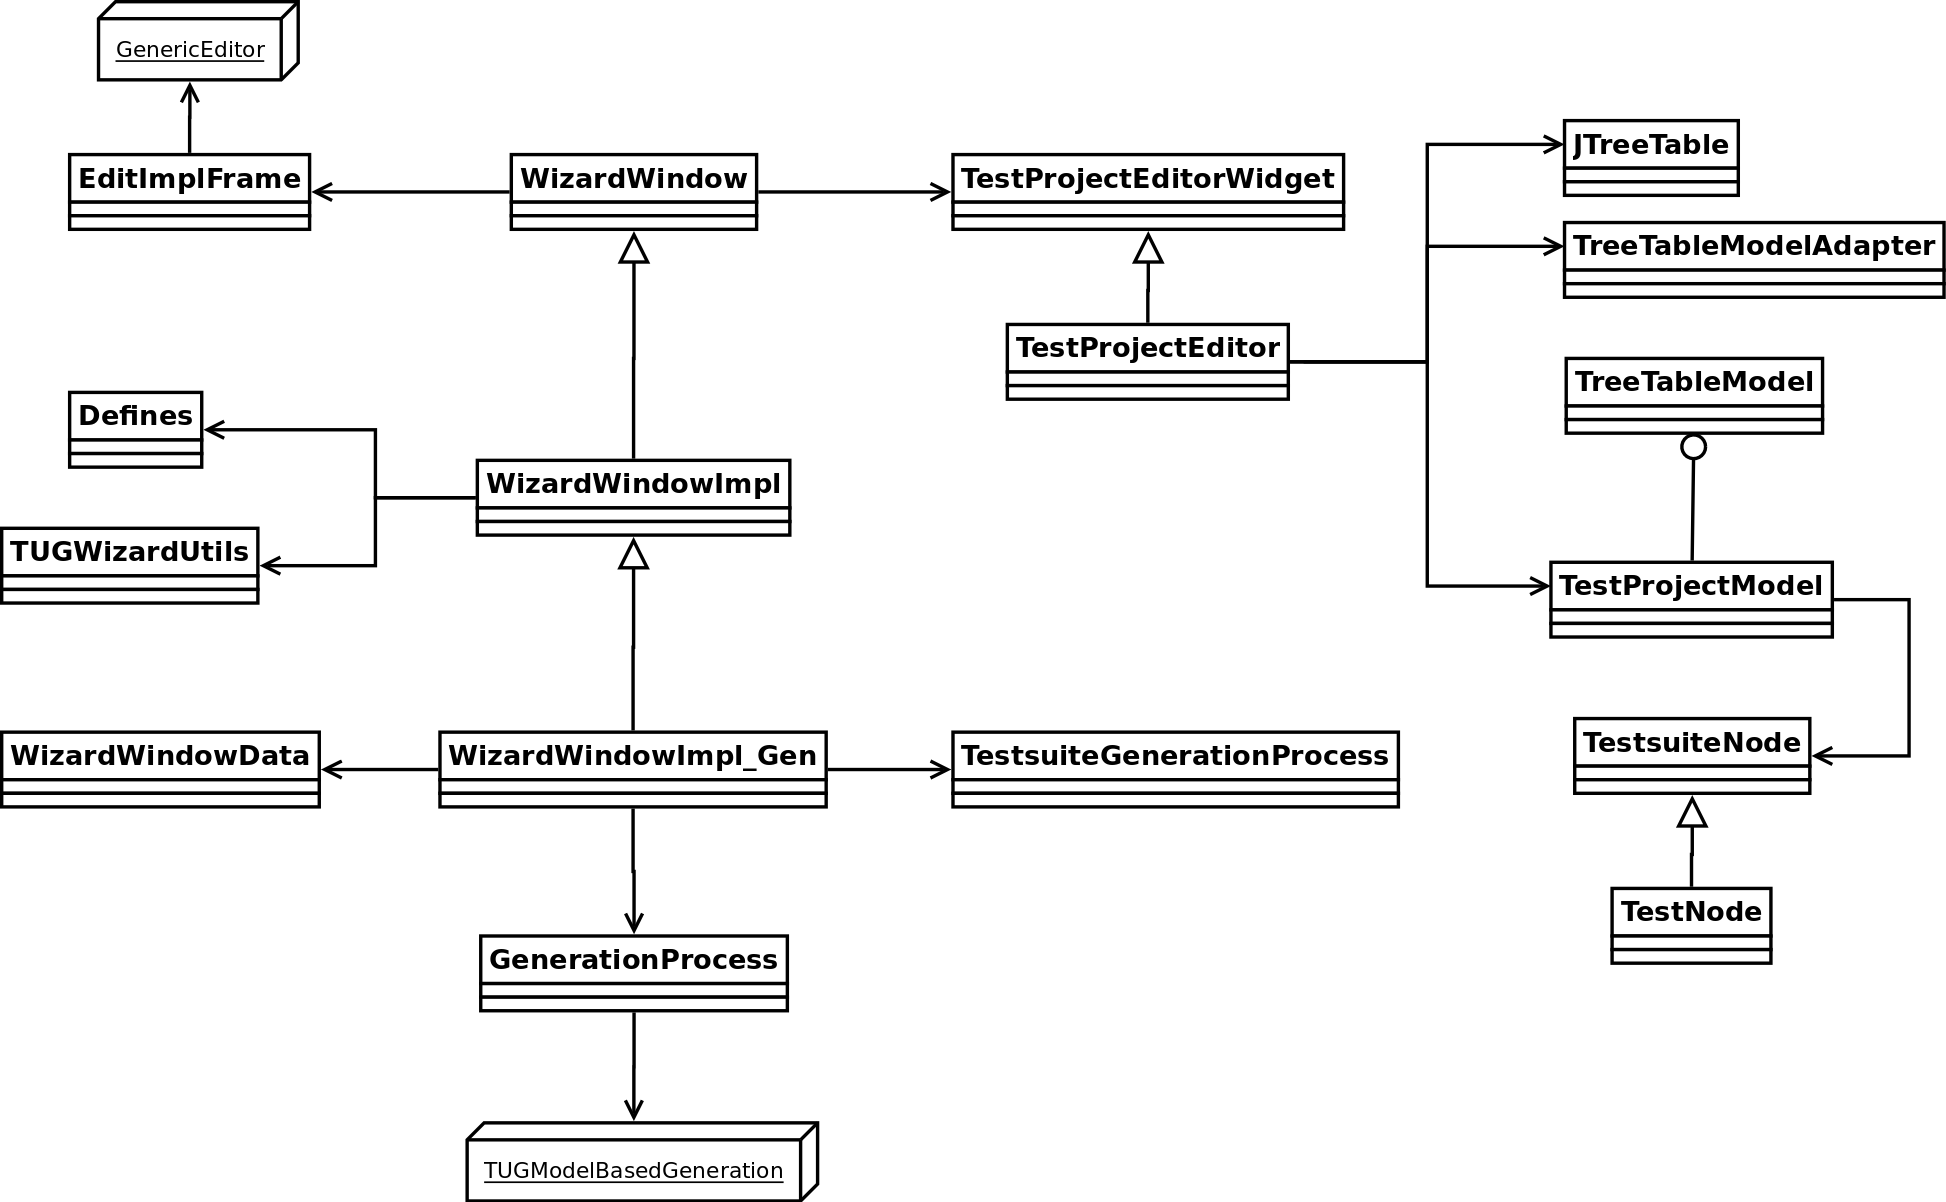
\includegraphics[width=.99\textwidth]{images/diag/tug_wizard_classdiag.png}
\vspace{2ex}

This architecture is divided into three levels. Inheritance is used to
divide the implementation of {\tt WizardWindow} into the following three
classes:
%
\begin{itemize}
\item {\tt WizardWindow}: includes configuration and deployment of TUG
  Wizard user interface.
%
\item {\tt WizardWindowImpl}: includes the implementation under the TUG
  Wizard user interface, excluding generation functionality.
%
\item {\tt WizardWindowImpl\_Gen}: includes the implementation of the
  test project generation processes.
\end{itemize}

The most relevant classes included at each of these levels are further
described in the following.

\newpage

%%%
%%% WizardWindow

As said above, \field{WizardWindow} implements the configuration and
deployment of TUG Wizard user interface. It uses two supporting classes,
\field{EditImplFrame} and \field{TestProjectEditorWidget}, used to allow
developers to edit configuration files and to configure a test project
structure, respectively.  


\field{EditImplFrame} is the main class of \field{GenericEditor}, an
external component used in TUG Wizard in Steps 4 and 5 to allow the
modification of configuration files. This component is not further
described because it is out of the scope of this guide.


\vspace{2ex}
\begin{center}
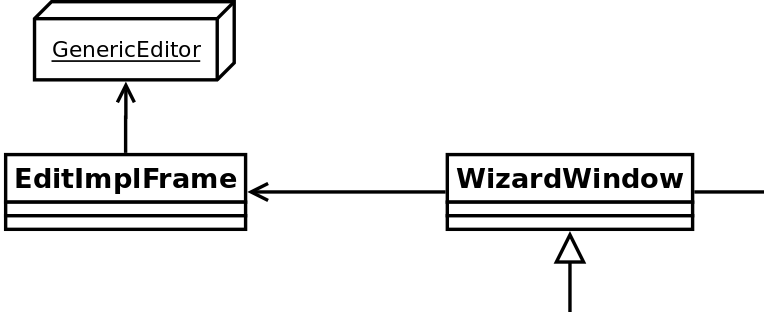
\includegraphics[width=.65\textwidth]{images/diag/tug_wizard_classdiag_ww1.png}
\end{center}
\vspace{2ex}


\field{TestProjectEditorWidget} represents the component to configure a
test project structure composed of a set of testsuites and tests (Step 6 in
TUG Wizard). The editor is based on a \field{JTreeTable} object and uses an
underlying model described by \field{TestProjectModel}.


\vspace{2ex}
\begin{center}
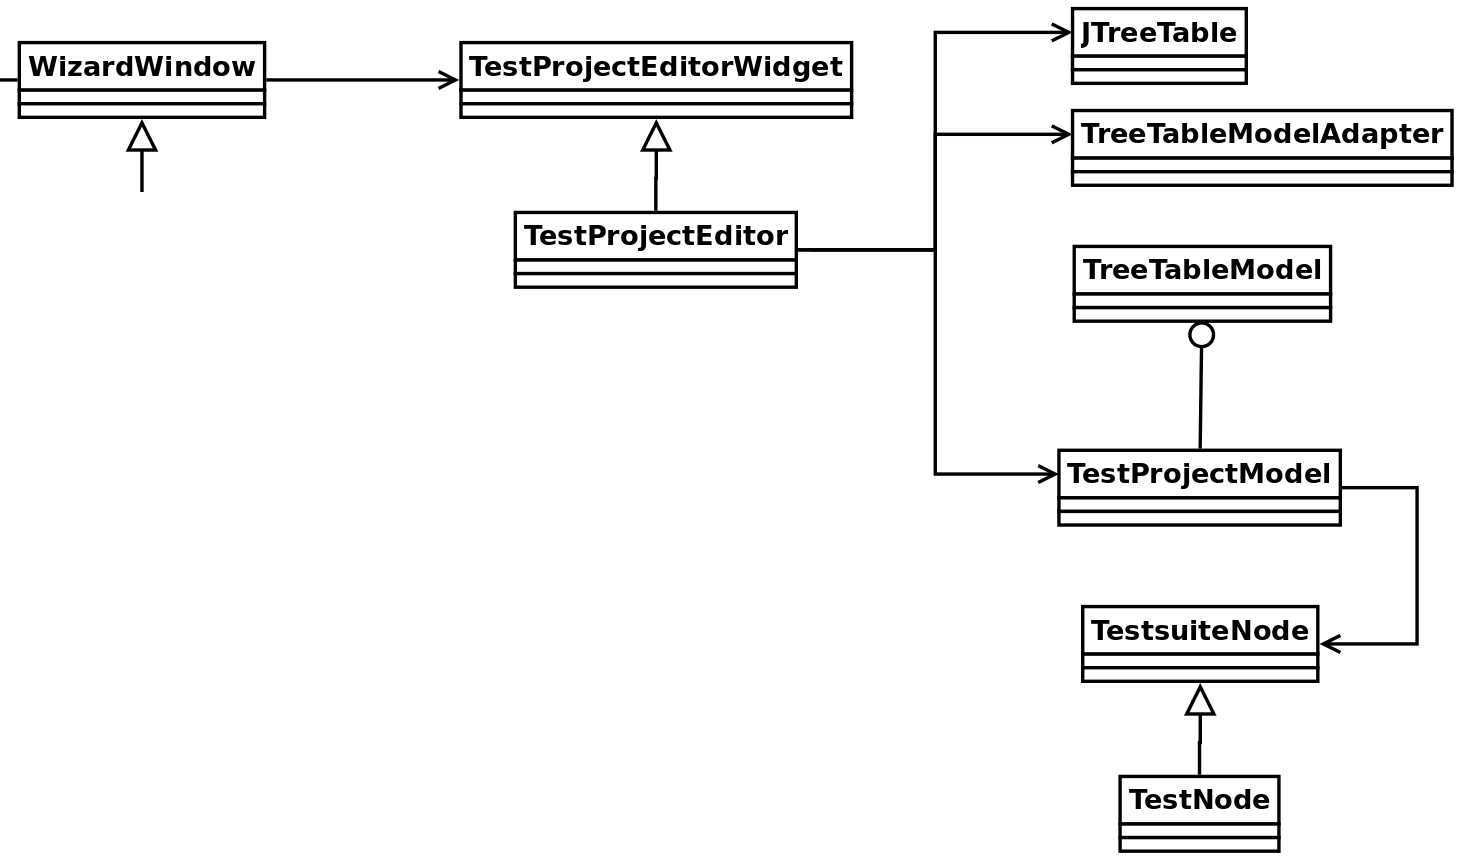
\includegraphics[width=.99\textwidth]{images/diag/tug_wizard_classdiag_ww2.png}
\end{center}
\vspace{2ex}


%%%
%%% WizardWindowImpl

\field{WizardWindowImpl} includes all the implementation under the TUG
Wizard user interface. It implements all steps in the process, excluding
Step 7 in which the generation process is carried out.

\field{TUGWizardUtils} implements supporting methods to simplify the wizard
processes.
%
The \field{Defines} class defines some constant values used during the
wizard and generation processes.


\vspace{2ex}
\begin{center}
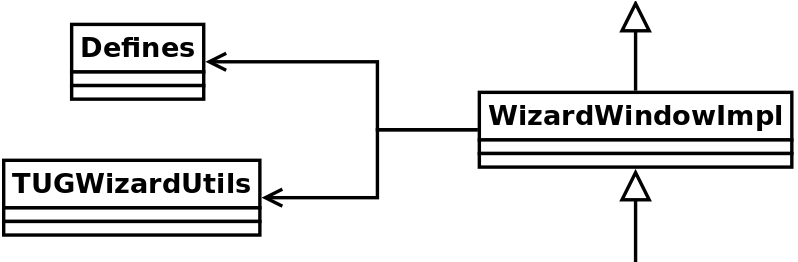
\includegraphics[width=.65\textwidth]{images/diag/tug_wizard_classdiag_wwi1.png}
\end{center}
\vspace{2ex}


%%%
%%% WizardWindowImpl\_Gen

\field{WizardWindowImpl\_Gen} includes all the implementation of the TUG
Wizard related to the test project generation processes. 


\vspace{2ex}
\begin{center}
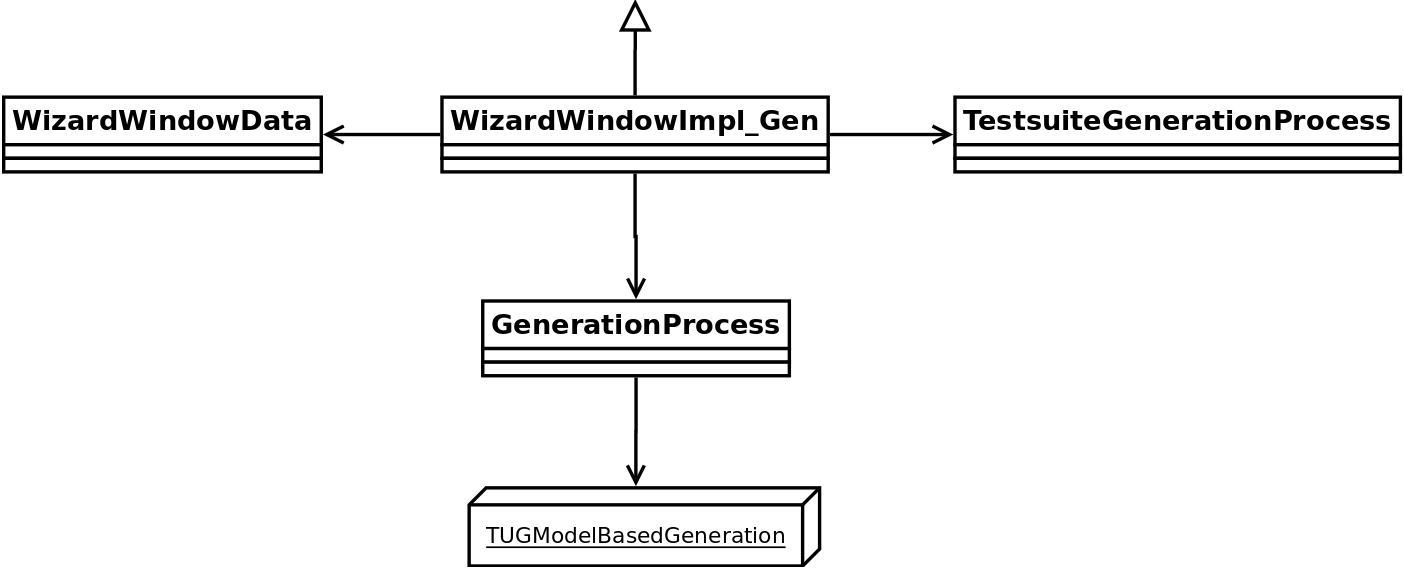
\includegraphics[width=.99\textwidth]{images/diag/tug_wizard_classdiag_wwig1.png}
\end{center}
\vspace{2ex}


The generation processes are based on the data encapsulated within
\field{WizardWindowData}. This object includes all configuration data
provided by developers during the wizard steps.


%%%
\field{GenerationProcess} encapsulates the generation of a new test panel
project. This process uses the Qt panel and the dependencies introduced by
developers in the wizard steps to generate a new panel to be tested.
%
This new panel inherits the original one and includes methods to simulate
users interaction with the widgets composing the panel. These methods are
aimed at being used in tests definition.
%
It is also generated a Qt project to compile and run this panel standalone.


%%%
The \field{TestsuiteGenerationProcess} class includes methods supporting
the generation of a test project structure. A test project is composed of:
%
\begin{itemize}
\item a main project called {\tt build\_all.pro} from which everything can
  be compiled.
\item the test panel project described above. It is included in {\tt
  \_main} folder. 
\item a set of testsuites. Each testsuite includes a set of empty methods
  (i.e., the tests) to be filled by developers with the desired
  functionality. Methods from the test panel and from {\tt qt\_TestUtils}
  class can be used to support the tests implementation.
\item a Qt project for each testsuite. This project can be used to compile
  and run the testsuites standalone.
\end{itemize}



%%%
%%%


%\begin{lstlisting}
%xxxx
%\end{lstlisting}



\newpage


%%% Local variables:
%%% mode: latex
%%% TeX-master: "README.tex"
%%% ispell-local-dictionary: "american"
%%% coding: utf-8
%%% fill-column: 75
%%% TeX-parse-self: t
%%% TeX-auto-save: t
%%% End:


\subsection{Wizard Configuration}

TUG Wizard includes some files that allow developers to configure the
generation process. Some of these files can be modified from the TUG Wizard
user interface. Others can only be modified using an external text editor.
%
These files can be found in {\tt config/} folder, and are briefly described
in the following. 

%%
%%
{\tt config/generation\_templates}: set of templates used during the
generation of testsuites and test projects.
\begin{itemize}
%
\item {\tt testsuitebase\_template}: testsuite base template.
\item {\tt mp\_testsuite\_template}: template for testsuites in which a new
  panel is launched for each test.
\item {\tt mp\_test\_template}: template for tests in which a new panel is
  launched for each test.
\item {\tt op\_testsuite\_template}: template for testsuites in which only
  one panel is used to execute all tests (for leaf nodes in the test
  projects structure).
\item {\tt op\_testsuite\_internal\_template}: template for testsuites in
  which only one panel is used to execute all tests (for internal nodes in
  the test projects structure).
\item {\tt op\_test\_template}: template for tests in which only one panel
  is used to execute all tests.
\item {\tt testsuite\_project\_main}: template for main file launching a testsuite.           
\item {\tt testsuite\_project\_pro}: template for Qt project file compiling
  a testsuite.
%
\end{itemize}


%%
%%
{\tt config/includes}: set of files in which the includes related to
different options selected in TUG Wizard are defined. These files can be
modified also from TUG Wizard user interface.
\begin{itemize}
%
\item {\tt boost\_signals\_include}: defines the lines to include Boost
  signals into a test project.
\item {\tt libsig\_signals\_include}: defines the lines to include Libsig
  signals into a test project.
\item {\tt gcov\_include}: defines the lines to include Gcov into a test
  project.
\item {\tt gprof\_include}: defines the lines to include Gprof into a test
  project.
\item {\tt tuglib\_include}: defines the lines to include TUGLib library
  into a test project.
%
\end{itemize}
  


\newpage

%%% Local variables:
%%% mode: latex
%%% TeX-master: "README.tex"
%%% ispell-local-dictionary: "american"
%%% coding: utf-8
%%% fill-column: 75
%%% TeX-parse-self: t
%%% TeX-auto-save: t
%%% End:




%%% Local variables:
%%% mode: latex
%%% TeX-master: "README.tex"
%%% ispell-local-dictionary: "american"
%%% coding: utf-8
%%% fill-column: 75
%%% TeX-parse-self: t
%%% TeX-auto-save: t
%%% End:



\end{document}

%%% Local variables:
%%% mode: latex
%%% TeX-master: "README.tex"
%%% ispell-local-dictionary: "american"
%%% coding: utf-8
%%% fill-column: 75
%%% TeX-parse-self: t
%%% TeX-auto-save: t
%%% End:
